z


%%%%%%%%%%%%%%%%%%%%%%%%%%%%%%%%%%%%%%%%%%%%%%%%%%%%%%%%%%%%%%%%%%%%%%%%%%%%%%%%
% Thesis / Project Report
% LaTeX Template
% Version 2.0 (08/04/16)
%
% Author:
% Parth Ganeriwala
% https://github.com/ParthGaneriwala/BITS-Thesis-Template-Latex
%
% This template is heavily based on the work of Siddhant Shrivastava, Darshit Shah, Steven Gunn and Sunil Patel
% Siddhant Shrivastava
% https://github.com/sidcode/bits-pilani-thesis-template-latex
% Darshit Shah
% https://github.com/darnir/BPHC-LaTeX-Report-Class
% Steven Gunn
% http://users.ecs.soton.ac.uk/srg/softwaretools/document/templates/
% and
% Sunil Patel
% http://www.sunilpatel.co.uk/thesis-template/
%
% License:
% CC BY-NC-SA 4.0 (http://creativecommons.org/licenses/by-nc-sa/4.0/)
%
% Note:
% Make sure to edit document variables in the Thesis.cls file
%
%%%%%%%%%%%%%%%%%%%%%%%%%%%%%%%%%%%%%%%%%%%%%%%%%%%%%%%%%%%%%%%%%%%%%%%%%%%%%%%%

%-------------------------------------------------------------------------------
%	PACKAGES AND OTHER DOCUMENT CONFIGURATIONS
%-------------------------------------------------------------------------------

\documentclass[11pt, a4paper, oneside, british]{Thesis} % Paper size, default font size
                                               % and one-sided paper

\graphicspath{{Figures}} % Specifies the directory where pictures are stored

\usepackage[sorting=none,bibstyle=numeric-comp,citestyle=numeric,backend=bibtex,defernumbers=true]{biblatex}  
\addbibresource{References.bib} % Specifies the bibliography file to be used 
\usepackage{physics}  
\usepackage{float} 
\usepackage{bookmark}  
\usepackage{multirow}  
\usepackage{booktabs, makecell}  
\usepackage[table, svgnames]{xcolor}  
\usepackage{siunitx}  
\usepackage{colortbl}  
\usepackage{wrapfig}  
\usepackage{bbm}  
\usepackage{ragged2e}  
\usepackage{array}  
\usepackage{scalerel}  
\usepackage{hyperref}  
\usepackage{mdframed}
\usepackage{cleveref}
\usepackage{tcolorbox}
\definecolor{Gray}{gray}{0.9}  
\newlength\mysep   
\setlength\mysep{1cm}  
\DeclareFloatSeparators{mysep}{\hskip\mysep}  

\AtBeginDocument{\RenewCommandCopy\qty\SI}  
\ExplSyntaxOn  
\msg_redirect_name:nnn { siunitx } { physics-pkg } { none }  
\ExplSyntaxOff  

\title{\ttitle}
\makeatletter  
\pdfstringdefDisableCommands{\let\HyPsd@CatcodeWarning\@gobble}  
\makeatother  

\usepackage[T1]{fontenc}
\begin{document}

\frontmatter % Use roman numbering style (i, ii...) for the pre-content pages

\setstretch{1.3} % Line spacing of 1.3

% Define page headers using FancyHdr package and set up for one-sided printing
\fancyhead{} % Clears all page headers and footers
\rhead{\thepage} % Sets the right side header to show the page number
\lhead{} % Clears the left side page header

\pagestyle{fancy} % Finally, use the "fancy" page style to implement the
                  %FancyHdr headers

% Input all the variables used in the document. Please fill out the
% variables.tex file with all your details.
%-------------------------------------------------------------------------------
%	DOCUMENT VARIABLES
%
%	Fill in the lines below to set the various variables for the document
%-------------------------------------------------------------------------------

%-------------------------------------------------------------------------------
% Your thesis title - this is used in the title and abstract
% Command: \ttitle
\thesistitle{Bachelor Thesis}
%-------------------------------------------------------------------------------
% The document type: Thesis / report, etc.
% Command: \doctype
\documenttype{Undergraduate Thesis}
%-------------------------------------------------------------------------------
% Your supervisor's name - this is used in the title page
% Command: \supname
\supervisor{Henry \textsc{Pinto}}
%-------------------------------------------------------------------------------
% The supervisor's position - Used on Certificate
% Command: \suppos
\supervisorposition{Associate PhD Professor}
%-------------------------------------------------------------------------------
% Supervisor's institute
% Command: \supinst
\supervisorinstitute{Yachay Tech University}
\supervisorinstitutecountry{Urcuqui, Ecuador}
%-------------------------------------------------------------------------------
% Your Co-Supervisor's name
% Command: \cosupname
\cosupervisor{Andres \textsc{Garay}}
%-------------------------------------------------------------------------------
% Co-Supervisor's Position - Used on Certificate
% Command: \cosuppos
\cosupervisorposition{Associate PhD Professor}
%-------------------------------------------------------------------------------
% Co-Supervisor's Institute
% Command: \cosupinst
\cosupervisorinstitute{Centro de Investigacion en Materiales Avanzados}
\cosupervisorinstitutecountry{Monterrey, Mexico}
%-------------------------------------------------------------------------------
% Your Examiner's name. Not currently used anywhere.
% Command: \examname
\examiner{}
%-------------------------------------------------------------------------------
% Name of your degree
% Command: \degreename
\degree{Bachelor of Physics}
%-------------------------------------------------------------------------------
% The BITS Course Code for which this report is written
% COmmand: \ccode
\coursecode{BITS F421T}
%-------------------------------------------------------------------------------
% The name of the Course
% Command: \cname
\coursename{Thesis}
%-------------------------------------------------------------------------------
% Your name. Extend manually in case of multiple authors
% Command: \authornames
\authors{J. Gabriel \textsc{Balarezo}}
%-------------------------------------------------------------------------------
% Your ID Number - used on the Title page and abstract
% Command: \idnum
\IDNumber{0106019219}
%-------------------------------------------------------------------------------
% Your address
% Command: \addressnames
\addresses{}
%-------------------------------------------------------------------------------
% Your subject area
% Command: \subjectname
\subject{}
%-------------------------------------------------------------------------------
% Keywords for this report.
% Command: \keywordnames
\keywords{Ab initio calculations, electronic properties, magnetic properties, XGeTe$_3$ monolayers, VASP, PBE,PBESol, Phonopy, Alloy-Theoretic Automated Toolkit, Hubbard U corrections.}
%-------------------------------------------------------------------------------
% University details
% Command: \univname
\university{\texorpdfstring{\href{https://www.bits-pilani.ac.in/Dubai/index.aspx} % URL
                {Yachay Tech University}} % University name
                {Yachay Tech University}}
%-------------------------------------------------------------------------------
% University details, in Capitals
% Command: \UNIVNAME
\UNIVERSITY{\texorpdfstring{\href{https://www.bits-pilani.ac.in/Dubai/index.aspx} % URL
                {Yachay Tech University}} % name in capitals
                {Yachay Tech University}}
                
\UNIVERSITYCOUNTRY{\texorpdfstring{Urcuqui, Ecuador}}
%-------------------------------------------------------------------------------
% Department Details
% Command: \deptname
%\department{\texorpdfstring{\href{https://www.bits-pilani.ac.in/dubai/computerscience/DetofComputerScience} % Your department's URL
%                {Computer Science}} % Your department's name
%                {Computer Science}}
%-------------------------------------------------------------------------------
% Department details, in Capitals
% Command: \DEPTNAME
%\DEPARTMENT{\texorpdfstring{\href{https://www.bits-pilani.ac.in/dubai/computerscience/DetofComputerScience} % Your department's URL
%                {Computer Science}} % Your department's name in capitals
%                {Computer Science}}
%-------------------------------------------------------------------------------
% Research Group Details
% Command: \groupname
\group{\texorpdfstring{\href{Research Group Web Site URL Here (include http://)}
                {Research Group Name}} % Your research group's name
                {Research Group Name}}
%-------------------------------------------------------------------------------
% Research Group Details, in Capitals
% Command: \GROUPNAME
\GROUP{\texorpdfstring{\href{Research Group Web Site URL Here (include http://)}
                {RESEARCH GROUP NAME (IN BLOCK CAPITALS)}}
                {RESEARCH GROUP NAME (IN BLOCK CAPITALS)}}
%-------------------------------------------------------------------------------
% Faculty details
% Command: \facname
\faculty{\texorpdfstring{\href{Faculty Web Site URL Here (include http://www.yachaytech.edu.ec/en/physicsandnanotech/)}
                {School of Physical Sciences and Nanotechnology}}
                {School of Physical Sciences and Nanotechnology}}
%-------------------------------------------------------------------------------
% Faculty details, in Capitals
% Command: \FACNAME
\FACULTY{\texorpdfstring{\href{Faculty Web Site URL Here (include http://)}
                {FACULTY NAME (IN BLOCK CAPITALS)}}
                {FACULTY NAME (IN BLOCK CAPITALS)}}
%-------------------------------------------------------------------------------


%-------------------------------------------------------------------------------
%   NON-CONTENT PAGES
%-------------------------------------------------------------------------------
\maketitle

\Authorship

\Declaration

\Dedicatory{For her, who is my everything.\\
For my family, who always supported me.\\} 

\Acknowledgements

\Resumen

\Abstract



% \Quotation{Insert Random Quote here. Publish like a boss.}{Your Name}





%-------------------------------------------------------------------------------
%	LIST OF CONTENTS/FIGURES/TABLES PAGES
%-------------------------------------------------------------------------------

% The page style headers have been "empty" all this time, now use the "fancy"
% headers as defined before to bring them back
\pagestyle{fancy}

\lhead{\emph{Contents}} % Set the left side page header to "Contents"
\tableofcontents % Write out the Table of Contents

% Set the left side page header to "List of Figures"
\lhead{\emph{List of Figures}}
\listoffigures % Write out the List of Figures

 % Set the left side page header to "List of Tables"
\lhead{\emph{List of Tables}}
\listoftables % Write out the List of Tables

%-------------------------------------------------------------------------------
%	ABBREVIATIONS
%-------------------------------------------------------------------------------


%-------------------------------------------------------------------------------
%	PHYSICAL CONSTANTS/OTHER DEFINITIONS
%-------------------------------------------------------------------------------

% \clearpage % Start a new page

% % Set the left side page header to "Physical Constants"
% \lhead{\emph{Physical Constants}}

%  % Include a list of Physical Constants (a four column table)
% \listofconstants{lrcl}
% {
% Speed of Light & $c$ & $=$ & $2.997\ 924\ 58\times10^{8}\ \mbox{ms}^{-\mbox{s}}$ (exact)\\
% % Constant Name & Symbol & = & Constant Value (with units) \\
% }

%-------------------------------------------------------------------------------
%	SYMBOLS
%-------------------------------------------------------------------------------

% \clearpage % Start a new page

% \lhead{\emph{Glossary}} % Set the left side page header to "Symbols"

% \listofnomenclature % List the nomenclature. (We use the glossaries package)

%-------------------------------------------------------------------------------
%	DEDICATION
%-------------------------------------------------------------------------------

\mainmatter % Begin numeric (1,2,3...) page numbering

\pagestyle{fancy} % Return the page headers back to the "fancy" style

% Include the chapters of the thesis as separate files from the Chapters folder
% Uncomment the lines as you write the chapters

% Chapter Template

\chapter{Introduction} % Main chapter title

\label{Chapter1} % Change X to a consecutive number; for referencing this chapter elsewhere, use \ref{ChapterX}

\lhead{Chapter 1. \emph{Introduction}} % Change X to a consecutive number; this is for the header on each page - perhaps a shortened title

%----------------------------------------------------------------------------------------
%	SECTION 1
%----------------------------------------------------------------------------------------

%############################# Introduction #################################
\section{Background}
  Concrete is the synthetic material currently produced in volumes larger than any other material on Earth. With an annual consumption of approximately 35 billion tonnes, it is only second to water in terms of global usage\supercite{Monteiro2017, VanDamme2018}. As the backbone of modern infrastructure, it provides the foundations for buildings, bridges, roads, dams, and other structures essential for societal development. Its widespread adoption arises from a unique combination of strength, versatility, and cost-effectiveness\supercite{Mehta2014}, rendering it indispensable to the construction industry.

  Nevertheless, despite the ubiquity of concrete, the properties of its key constituent, cement, remain incompletely understood. Cement is a chemically complex material, composed of a heterogeneous mixture of minerals that undergo a series of hydration reactions upon contact with water. The principal product of cement hydration---and the primary binding phase of concrete--- calcium silicate hydrate (C-S-H)\footnote{Cement chemistry nomenclature} is the responsible for the mechanical strength, chemical and transport properties and durability of hardened cement paste and, consequently, of concrete itself\supercite{Papatzani2015, Ioannidou2016, Qomi2020, Bahraq2022}. Therefore, understanding the atomic and mechanical properties of C-S-H is of the uttermost importance to better formulate cementitious materials with enhanced performance and durability.\supercite{Foley2012}



%-----------------------------------
%	SUBSECTION 1
%-----------------------------------
\section{Problem Statement}

Nunc posuere quam at lectus tristique eu ultrices augue venenatis. Vestibulum ante ipsum primis in faucibus orci luctus et ultrices posuere cubilia Curae; Aliquam erat volutpat. Vivamus sodales tortor eget quam adipiscing in vulputate ante ullamcorper. Sed eros ante, lacinia et sollicitudin et, aliquam sit amet augue. In hac habitasse platea dictumst.

%-----------------------------------
%	SUBSECTION 2
%-----------------------------------

\section{General and Specific Objectives}
Morbi rutrum odio eget arcu adipiscing sodales. Aenean et purus a est pulvinar pellentesque. Cras in elit neque, quis varius elit. Phasellus fringilla, nibh eu tempus venenatis, dolor elit posuere quam, quis adipiscing urna leo nec orci. Sed nec nulla auctor odio aliquet consequat. Ut nec nulla in ante ullamcorper aliquam at sed dolor. Phasellus fermentum magna in augue gravida cursus. Cras sed pretium lorem. Pellentesque eget ornare odio. Proin accumsan, massa viverra cursus pharetra, ipsum nisi lobortis velit, a malesuada dolor lorem eu neque.

%----------------------------------------------------------------------------------------
%	SECTION 2
%----------------------------------------------------------------------------------------

\section{Overview}

Sed ullamcorper quam eu nisl interdum at interdum enim egestas. Aliquam placerat justo sed lectus lobortis ut porta nisl porttitor. Vestibulum mi dolor, lacinia molestie gravida at, tempus vitae ligula. Donec eget quam sapien, in viverra eros. Donec pellentesque justo a massa fringilla non vestibulum metus vestibulum. Vestibulum in orci quis felis tempor lacinia. Vivamus ornare ultrices facilisis. Ut hendrerit volutpat vulputate. Morbi condimentum venenatis augue, id porta ipsum vulputate in. Curabitur luctus tempus justo. Vestibulum risus lectus, adipiscing nec condimentum quis, condimentum nec nisl. Aliquam dictum sagittis velit sed iaculis. Morbi tristique augue sit amet nulla pulvinar id facilisis ligula mollis. Nam elit libero, tincidunt ut aliquam at, molestie in quam. Aenean rhoncus vehicula hendrerit.

\begin{figure}[H]
    \centering
    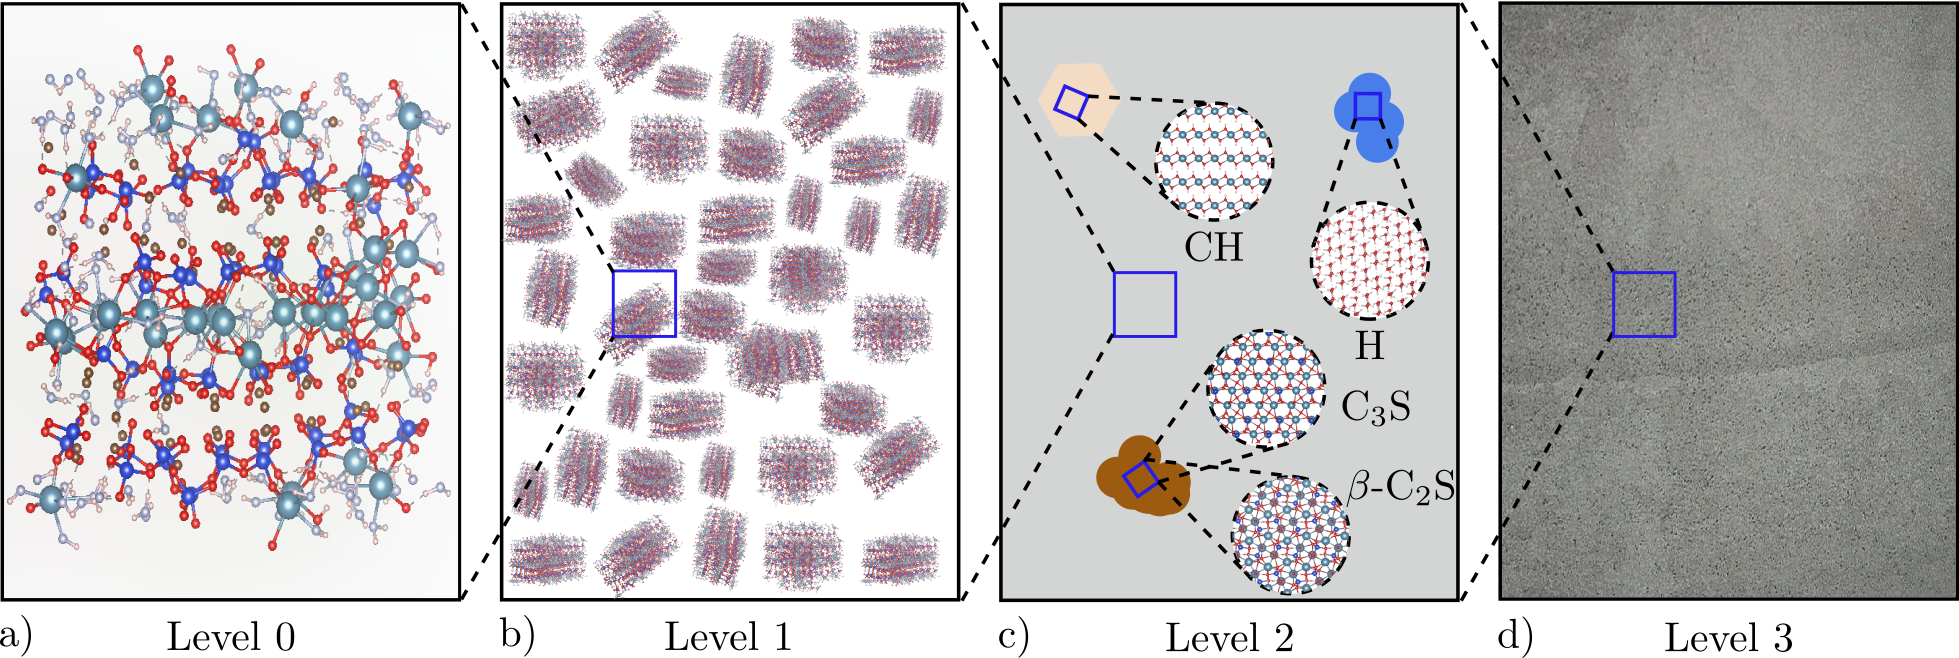
\includegraphics[width=0.8\textwidth]{levels.png}
    \caption{A four-level model representing the upscaling of C-S-H properties from the nanoscale to the engineering scale. (a) snapshot of C-S-H's nanostructure. (b) microstructure of C-S-H created by agglomeration of randomly oriented C-S-H nanoparticles. (c) microtexture of hardened paste composed by hydration products. (d) macrotexture of cement paste at the engineering scale. Adapted from \supercite{AbdolhosseiniQomi2015}.}
    \label{fig:figure1}
\end{figure}



% Chapter Template

\chapter{Theoretical Background} % Main chapter title

\label{Chapter2} % Change X to a consecutive number; for referencing this chapter elsewhere, use \ref{ChapterX}

\lhead{Chapter 2. \emph{Theoretical Background}}
This chapter is devoted to present the theoretical foundations and formalism of Density Functional Theory (DFT) and related methods required for the development of the results presented in this work. Starting with the many-body Schrödinger equation, this chapter covers the Born-Oppenheimer approximation, the Hartree-Fock approximation, Hohenberg-Kohn theorems, the Kohn-Sham equations, exchange-correlation functionals, and definitions on Ab initio molecular dynamics (AIMD) and machine learning force fields (MLFFs), along with implementation details in the Vienna Ab initio Simulation Package (VASP).

Ultimately, this chapter aims to provide a comprehensive understanding of the theoretical framework that underpins the computational methods utilised in this work, enabling the reader to grasp the principles and assumptions that govern the simulations and analyses performed throughout.

\section{Many Body Schrödinger Equation}
In the realm of materials science, comprehending particle behaviour within a system inevitably demands resorting to intricate principles of quantum mechanics. Our journey shall commence by describing the physical laws that shape the interactions among particles constituting a system---electrons and nuclei alike. 

\subsection{The Coulomb Interaction}

Materials may be thought of as complex assemblies of electrons and nuclei, held together by a delicate balance between attractive Coulomb interactions---primarily between electrons and nuclei---and repulsive interactions between like-charged particles, such as electron-electron and nucleus-nucleus pairs, which govern the overall dynamics of the material system\supercite{giustino2014materials, sholl2023density, kaxiras2003atomic}.  From classical electrostatics, these interactions can be mathematically expressed as follows: 

\begin{itemize}
\item Electron-electron interactions 
  \begin{equation}
    \label{eq1}
    \hat{V}_{ee} = \frac{1}{2} \sum_{i\neq j} \frac{e^2}{4\pi\epsilon_0 |\mathbf{r}_i - \mathbf{r}_j|}
  \end{equation}
\item Electron-nucleus interactions 
  \begin{equation}
    \label{eq2}
    \hat{V}_{nn} = \frac{1}{2} \sum_{I\neq J} \frac{e^2}{4\pi\epsilon_0} \frac{Z_I Z_J}{|\mathbf{R}_I - \mathbf{R}_J|}
  \end{equation}
\item Electron-nuclei interactions 
\begin{equation}
    \label{eq3}
    \hat{V}_{en} = -\sum_{i\neq I} \frac{e^2}{4\pi\epsilon_0} \frac{Z_I}{|\mathbf{r}_i - \mathbf{R}_I|}
  \end{equation}
\end{itemize}

where $e$ is the electronic charge, $\epsilon_0$ is the vacuum permittivity, $Z_I$ and $Z_J$ are the atomic numbers of nuclei $I$ and $J$, respectively, and $\mathbf{r}_i$ and $\mathbf{R}_I$ are the position vectors of electrons and nuclei, respectively. Moreover, we must also consider the kinetic energy of the collection of electrons and nuclei
\begin{equation}
    \label{eq4}
    \hat{T} = -\sum_i \frac{\hbar^2}{2m_e} \nabla_i^2 - \sum_I \frac{\hbar^2}{2M_I} \nabla_I^2
\end{equation}
where $\hbar$ is the reduced Planck's constant, $m_e$ is the electron mass, and $M_I$ is the mass of the nucleus $I$.

\subsection{The Time-Independent Schrödinger Equation}
The Time-Independent Schrödinger Equation (TISE) lies at the heart of non-relativistic quantum mechanics, providing a mathematical framework to describe stationary electronic states of quantum systems. It takes the following form:
\begin{equation}
  \label{eq5}
  \hat{H} \psi(\mathbf{r}) = E \psi(\mathbf{r})
\end{equation}
where $\hat{H}$ is the Hamiltonian of the system, encompassing both kinetic and potential energies, $\psi(\mathbf{r})$ is the wavefunction of the system, and $E$ is the energy eigenvalue associated with the state described by $\psi(\mathbf{r})$.  It is important to note that Equation \ref{eq5} is only applicable to a single particle, yet a material system is composed of many electrons (N) and nuclei (M) with spatial coordinates $\mathbf{r}_1, \mathbf{r}_2, \ldots, \mathbf{r}_N$ and $\mathbf{R}_1, \mathbf{R}_2, \ldots, \mathbf{R}_M$, respectively. Therefore, we must introduce a so-called many-body wavefunction given by:
\begin{equation}
  \Psi(\mathbf{r}_1, \mathbf{r}_2, \ldots, \mathbf{r}_N, \mathbf{R}_1, \mathbf{R}_2, \ldots, \mathbf{R}_M)
  \label{eq5b}
\end{equation}
On this basis, the many-body version of Equation \ref{eq5} shall be constructed by combining the kinetic (Equation \ref{eq4}) and potential (Equations \ref{eq1}, \ref{eq2}, and \ref{eq3}) energy contributions, leading to the following expression:
\begin{equation}
  \label{eq6}
  \begin{split}
    \left[
      -\sum_i \frac{\hbar^2}{2m_e} \nabla_i^2 
      - \sum_I \frac{\hbar^2}{2M_I} \nabla_I^2 
      + \frac{1}{2} \sum_{i\neq j} \frac{e^2}{4\pi\epsilon_0 |\mathbf{r}_i - \mathbf{r}_j|} +\right. \\
      \left. \frac{1}{2} \sum_{I\neq J} \frac{e^2}{4\pi\epsilon_0} \frac{Z_I Z_J}{|\mathbf{R}_I - \mathbf{R}_J|} 
      - \sum_{i, I} \frac{e^2}{4\pi\epsilon_0} \frac{Z_I}{|\mathbf{r}_i - \mathbf{R}_I|}
    \right]\Psi = E_{\text{tot}} \Psi
  \end{split}
\end{equation}
Equation \ref{eq6} provides a complete description of the stationary states of a non-relativistic many-body system, under time-independent conditions and in the absence of external fields. Additionally, we can achieve a more compact formulation by introducing the concept of atomic units. To this end, let us consider the simplest electron-nucleus system---the hydrogen atom---where the electron orbital has an average radius $a_0 \approx 0.529 \, \text{Å}$. Thereby, the Coulomb energy for such a system is given by:
\begin{equation}
  \label{eq7}
  E_{\text{Ha}} = \frac{e^2}{4 \pi \epsilon_0 a_0}
\end{equation}
where 'Ha' stands for Hartree. Within this framework, the Hartree energy represents the Coulomb interaction between two fundamental charges separated by a distance of one Bohr radius ($a_0$). Moreover, the angular momentum quantisation condition for the electron in the hydrogen atom is given by
\begin{equation}
  \label{eq8}
  m_e v a_0 = \hbar
\end{equation}
Additionally, the equilibrium condition between the nuclear attraction and the electron's centrifugal force can be expressed as:
\begin{equation}
  \label{eq9}
  \frac{e^2}{4 \pi \epsilon_0 a_0^2} = \frac{m_e v^2}{a_0}
\end{equation}
By combining Equations \ref{eq7}, \ref{eq8}, and \ref{eq9}, we derive the 
following relationships:
\begin{equation}
  \label{eq10}
  \frac{e^2}{4 \pi \epsilon_0 a_0} = \frac{\hbar^2}{m_e a_0^2}
\end{equation}
\begin{equation}
  \label{eq11}
  \frac{1}{2} m_e v^2 = \frac{1}{2}E_{\text{Ha}}
\end{equation}
This latter relation showcases that the kinetic energy is of the same order as $E_\text{Ha}$, rendering it convenient to normalise Equation \ref{eq6} by this quantity:
\begin{equation}
  \label{eq12}
  \begin{split}
    \left[
      -\sum_i \frac{1}{2}a_0^2 \nabla_i^2 
      - \sum_I \frac{1}{2} \frac{1}{(M_I/m_e)} \nabla_I^2 
      + \frac{1}{2} \sum_{i\neq j} \frac{a_0}{|\mathbf{r}_i - \mathbf{r}_j|}\right. \\
      \left. +  \frac{1}{2} \sum_{I\neq J} Z_I Z_J \frac{a_0}{|\mathbf{R}_I - \mathbf{R}_J|} 
      - \sum_{i, I} Z_I \frac{a_0}{|\mathbf{r}_i - \mathbf{R}_I|}
    \right]\Psi = \frac{E_{\text{tot}}}{E_{\text{Ha}}} \Psi
  \end{split}
\end{equation}
A final simplification involves setting our energy units to Ha, distance units to $a_0$, and mass units to $m_e$. The last missing constant $e$ is set to 1, leading to the following expression: 
\begin{equation}
  \label{eq13}
  \begin{split}
    \left[
      -\sum_i \frac{\nabla_i^2}{2}
      - \sum_I \frac{\nabla_I^2}{2 M_I} 
      + \frac{1}{2} \sum_{i\neq j} \frac{1}{|\mathbf{r}_i - \mathbf{r}_j|} + \right. \\
      \left. \frac{1}{2} \sum_{I\neq J} \frac{Z_I Z_J} {|\mathbf{R}_I - \mathbf{R}_J|} 
      - \sum_{i, I} \frac{Z_I}{|\mathbf{r}_i - \mathbf{R}_I|}
    \right]\Psi = E_{\text{tot}} \Psi
  \end{split}
\end{equation}

Ultimately, even though Equation \ref{eq13} provides an exact method capable of yielding various properties of a material system---such as elastic, thermal, and electronic properties---a combination of mathematical complexity and computational limitations renders it intractable to solve for any realistic system. Moreover, the wavefunction contains vastly more information than is necessary to describe most observable properties of a material. Therefore, we must resort to alternative formulations that allow us to extract only the relevant information from the wavefunction whilst reducing the computational cost of the calculations. The remainder of this chapter is dedicated to presenting such alternative approaches that ultimately lead to the computational methods employed throughout this work.

%-----------------------------------
%	SUBSECTION 1
%-----------------------------------
\section{The Born-Oppenheimer Approximation}
For atoms in a solid, we can think of nuclei as being held immobile in a fixed position, while electrons instantaneously react to any nucleus's movement. This assumption is based on the fact that nuclei are much heavier than electrons---by three to four orders of magnitude---making the former behave like classical particles. Thereby, we can rewrite the many-body wavefunction as a product of two wavefunctions:
\begin{equation}
  \Psi(\mathbf{r}_1, \mathbf{r}_2, \ldots, \mathbf{r}_N, \mathbf{R}_1, \mathbf{R}_2, \ldots, \mathbf{R}_M) = \psi_{\mathbf{R}}(\mathbf{r}_1, \mathbf{r}_2, \ldots, \mathbf{r}_N)\chi(\mathbf{R})
  \label{eq14}
\end{equation}
where $\psi_{\mathbf{R}}$ is the electronic wavefunction parametrised by the nuclear positions $\mathbf{R}$, and $\chi$ is the nuclear wavefunction. Furthermore, this significant mass disparity enables a systematic approximation scheme, in which the electronic wavefunction is solved for fixed nuclei, and its solution is used as an effective potential for the nuclear dynamics afterwards. First, nuclei' kinetic energy is neglected, as their positions are assumed to be fixed: 
\begin{equation}
  \label{eq15}
  \sum_I \frac{\nabla_I^2}{2 M_I} = 0
  \quad \text{and} \quad  E = E_{\text{tot}} - \sum_{I<J} \frac{Z_I Z_J}{|\mathbf{R}_I - \mathbf{R}_J|}
\end{equation}
Following, we define the Coulomb potential of the nuclei experienced by the electrons as:
\begin{equation}
  \label{eq16}
  V_{\text{n}}(\mathbf{r}) = - \sum_{I} \frac{Z_I}{|\mathbf{r} - \mathbf{R}_I|}
\end{equation}
Then, Equation \ref{eq13} can be rewritten as:
\begin{equation}
  \label{eq17}
  \left[
    -\sum_i \frac{\nabla_i^2}{2} + \sum_i V_{\text{n}}(\mathbf{r}_i) + \frac{1}{2} \sum_{i\neq j} \frac{1}{|\mathbf{r}_i - \mathbf{r}_j|} 
  \right] \Psi = E \Psi 
\end{equation}
Finally, by using Equation \ref{eq14}, we can define the electronic and nuclear Schrödinger equations as follows:
\begin{equation}
  \label{eq18}
  \left[
    -\sum_i \frac{\nabla_i^2}{2} + \sum_i V_{\text{n}}(\mathbf{r}_i) + \frac{1}{2} \sum_{i\neq j} \frac{1}{|\mathbf{r}_i - \mathbf{r}_j|} 
  \right] \psi_{\mathbf{R}} = E_{\mathbf{R}} \psi_{\mathbf{R}}
\end{equation}
\begin{equation}
  \label{eq19}
  \left[
    -\sum_I \frac{\nabla_I^2}{2 M_I} + \sum_{I<J} \frac{Z_I Z_J}{|\mathbf{R}_I - \mathbf{R}_J|} + E(\mathbf{R}_1,\dots,\mathbf{R}_M)\right] \chi(\mathbf{R}) = E_{\text{tot}} \chi(\mathbf{R})
\end{equation}
where $E_{\mathbf{R}}= E(\mathbf{R}_1,\dots,\mathbf{R}_M)$ is the electronic surface energy, which is a function of the nuclear positions, and serves as an effective potential shaping the nuclear dynamics. 

%-----------------------------------
%	SUBSECTION 2
%-----------------------------------

\section{Hartree-Fock Approximation}
The essence of the Hartree-Fock approximation (HFA) is to approximate the interacting many-electron system (Equation \ref{eq17}) by a set of non-interacting single-particle problems subject to an effective mean-field potential\supercite{martin2016interacting, helgaker2014molecular, feng2005introduction}. As a means to this, we first rewrite the total wavefunction for a system with N electrons as the product of single-electron wavefunctions---often referred to as the Hartree approximation\supercite{Hartree1928}---as showcased in Equation \ref{eq20}. 
\begin{equation}
  \Psi^H(\mathbf{r}_1, \dots, \mathbf{r}_N) = \prod_{i=1}^N \phi_i(\mathbf{r}_i)
  \label{eq20}
\end{equation}
Following, we construct the total energy functional as the expectation value of the Hamiltonian operator:
\begin{equation}
  \label{eq21}
\begin{aligned}
  E^{H}[\{\phi_i\}] &= \bigg\langle \Psi^H \bigg| \hat{H} \bigg| \Psi^H \bigg\rangle 
\end{aligned}
\end{equation}
Expanding Equation \ref{eq21}:
\begin{equation}
  \label{eq22}
  \begin{split}
    E^{H}[\{\phi_i\}] &= \sum^N_{i=1} \int \phi_i^*(\mathbf{r}) \left(-\frac{\nabla^2}{2} + V_{\text{n}}(\mathbf{r})\right) \phi_i(\mathbf{r}) d\mathbf{r}  + \frac{1}{2} \sum_{i\neq j} \int\int \frac{|\phi_i(\mathbf{r})|^2 |\phi_j(\mathbf{r'})|^2 }{|\mathbf{r} - \mathbf{r'}|} d\mathbf{r} d\mathbf{r'}
  \end{split}
\end{equation}
where the first term adds up the kinetic energy and electron-nuclear attraction overall electrons, whilst the second accounts for the classical electron-electron repulsion energy averaged over the electron density distribution. In order to find the set of orbitals $\{\phi_i\}$ that minimises the total energy functional, we use the variational principle where we shall impose the orthonormality condition: 
\begin{equation}
  \label{eq23}
  \int \phi_i^*(\mathbf{r}) \phi_j(\mathbf{r}) d\mathbf{r} = \delta_{ij}
\end{equation}
for what we introduce the Lagrange multipliers $\lambda_{ij}$ to enforce these constraints and define the Lagrangian:
\begin{equation}
  \label{eq24}
  \mathcal{L} = E^H[\{\phi_i\}] - \sum_{i=1}^{N}\lambda_{ij} ( \langle\phi_i|\phi_j\rangle - \delta_{ij})
\end{equation}
which ultimately simplifies to:
\begin{equation}
  \label{eq25}
  \mathcal{L} = E^H[\{\phi_i\}] - \sum_{i=1}^{N}\varepsilon_{i} ( \langle\phi_i|\phi_i\rangle - 1)
\end{equation}

Then, we need to compute the derivative of $\mathcal{L}$ with respect to $\phi_i^*$ and set it to zero:
\begin{equation}
  \label{eq26}
  \frac{\delta \mathcal{L}}{\delta \phi_i^*}(\mathbf{r}) = 0
\end{equation}
which yields to the Hartree equation:
\begin{equation}
  \label{eq27}
  \left[-\frac{\nabla^2}{2} + V_{\text{n}}(\mathbf{r}) + V^H_i(\mathbf{r})\right]\phi_i(\mathbf{r})  = \varepsilon_i \phi_i(\mathbf{r})
\end{equation}
where $V_n(\mathbf{r})$ represents the electrostatic interaction between electrons and nuclei, and the Hartree potential 
\begin{equation}
  \label{eq28}
  V^H_i(\mathbf{r}) = \sum_{j\neq i} \int \frac{|\phi_j(\mathbf{r'})|^2}{|\mathbf{r} - \mathbf{r'}|} d\mathbf{r'}
\end{equation}
accounts for the average electrostatic interaction experienced by the $i$-th electron due to all other electrons in the system. This effective mean-field potential replaces the electron-electron interactions, effectively simplifying the many-body problem into single-particle problems. 
\subsection{The Pauli Exclusion Principle}
So far, we have introduced the Hartree approximation, which assumes that the many-electron wavefunction can be expressed as a product of single-particle wavefunctions. However, this approach does not account for the indistinguishability of electrons and the Pauli exclusion principle, which states that no two fermions--- half-spin particles, such as electrons---can reside in the same quantum state simultaneously. In doing so, it imposes a restriction on the possible configurations of electrons in a system that shall be accounted for.
 
 In order to achieve this, V. Fock\supercite{Fock1930} introduced a different approximation to the wavefunction by using a Slater determinant---a mathematical construct that combines one-electron wavefunctions in such a way that satisfies the antisymmetry principle. This is done by expressing the overall wavefunction as the determinant of a matrix of single-electron wavefunctions:
\begin{equation}
  \Psi^{HF}(\mathbf{r}_1, \dots, \mathbf{r}_N) = \frac{1}{\sqrt{N!}} \begin{vmatrix}
    \phi_1(\mathbf{r}_1) & \phi_1(\mathbf{r}_2) & \dots & \phi_1(\mathbf{r}_N)\\
    \phi_2(\mathbf{r}_1) & \phi_2(\mathbf{r}_2) & \dots & \phi_2(\mathbf{r}_N)\\
    \vdots & \vdots & \ddots & \vdots\\
    \phi_N(\mathbf{r}_1) & \phi_N(\mathbf{r}_2) & \dots & \phi_N(\mathbf{r}_N)
  \end{vmatrix}
  \label{eq29}
\end{equation}
where $1/\sqrt{N!}$ is a normalisation factor. To illustrate this, consider a two-electron system with single-particle wavefunctions $\phi_1(\mathbf{r})$ and $\phi_2(\mathbf{r})$. The Slater determinant for this system would be:
\begin{equation}
  \Psi^{HF}(\mathbf{r}_1, \mathbf{r}_2) = \frac{1}{\sqrt{2}} \begin{vmatrix}
    \phi_1(\mathbf{r}_1) & \phi_1(\mathbf{r}_2)\\
    \phi_2(\mathbf{r}_1) & \phi_2(\mathbf{r}_2)
  \end{vmatrix} = \frac{1}{\sqrt{2}} \left[\phi_1(\mathbf{r}_1)\phi_2(\mathbf{r}_2) - \phi_1(\mathbf{r}_2)\phi_2(\mathbf{r}_1))\right]
  \label{eq30}
\end{equation}
Evidently, $\Psi^{HF}(\mathbf{r}_1, \mathbf{r}_2) = -\Psi^{HF}(\mathbf{r}_2, \mathbf{r}_1)$, which satisfies the antisymmetr principle. 
\subsection{The Hartree-Fock Equations}
The Hartree-Fock equations are derived in a similar manner we addressed the Hartree equations. We first define the total energy with the Hartree-Fock wavefunction (Equation \ref{eq29}) 
\begin{equation}
  \label{eq31}
  \begin{split}
    E^{HF}[\{\phi_i\}] &= \bigg\langle \Psi^{HF} \bigg| \hat{H} \bigg| \Psi^{HF} \bigg\rangle\\
    &= \sum_{i} \langle \phi_i \big|\frac{\nabla^2}{2} + V_{\text{n}}(\mathbf{r})\big| \phi_i \rangle\\
    &+ \frac{1}{2} \sum_{i\neq j} \langle \phi_i \phi_j \big| \frac{1}{|\mathbf{r}_i - \mathbf{r}_j|} \big| \phi_i \phi_j\rangle\\
    &- \frac{1}{2} \sum_{i\neq j} \langle \phi_i \phi_j \big| \frac{1}{|\mathbf{r}_i - \mathbf{r}_j|} \big| \phi_j \phi_i\rangle
  \end{split}
\end{equation}
Consequently, using the variational principle, we derive the Hartree-Fock equations: 
\begin{equation}
  \label{eq32}
  \left[-\frac{\nabla^2}{2} + V_{\text{n}}(\mathbf{r}) + V^H_i(\mathbf{r}) +\right]\phi_i(\mathbf{r})
  - \sum_{j\neq i} \langle \phi_j \big| \frac{1}{|\mathbf{r}_i - \mathbf{r}_j|} \big| \phi_i \rangle \phi_j(\mathbf{r})
  = \varepsilon_i \phi_i(\mathbf{r})
\end{equation}
Noticeably, Equation \ref{eq32} has an extra term compared with the Hartree equation (Equation \ref{eq27}). This term is called the "exchange" term\supercite{kaxiras2003atomic}, and describes the effects of exchange between electrons. It is convenient to try to express the Hartree-Fock equations in a more compact form, so we define the single-particle and total densities as 
\begin{equation}
  \label{eq33}
  \rho_i(\mathbf{r}) = |\phi_i(\mathbf{r})|^2
\end{equation}
\begin{equation}
  \label{eq34}
  \rho(\mathbf{r}) = \sum_i \rho_i(\mathbf{r}) 
\end{equation}
so the Hartree potential can be expressed as 
\begin{equation}
  \label{eq35}
  V^H_i(\mathbf{r}) = \sum_{j\neq i}  \int \frac{\rho_j(\mathbf{r'})}{|\mathbf{r} - \mathbf{r'}|} d\mathbf{r'} 
  = \int \frac{\rho(\mathbf{r'}) - \rho_i(\mathbf{r'})}{|\mathbf{r} - \mathbf{r'}|} d\mathbf{r'}
\end{equation}
Therefore, the single-particle exchange density can be constructed as 
\begin{equation}
  \label{eq36}
  \rho^X_i(\mathbf{r}, \mathbf{r'}) = \sum_{j\neq i}\frac{\phi_i(\mathbf{r'})\phi^*_i(\mathbf{r})\phi_j(\mathbf{r})\phi^*_j(\mathbf{r'})}{\phi_i(\mathbf{r})\phi^*_i(\mathbf{r})}
\end{equation}
Finally, the Hartree-Fock equations take the form 
\begin{equation}
  \label{eq37}
  \left[-\frac{\nabla^2}{2} + V_{\text{n}}(\mathbf{r}) + V^H_i(\mathbf{r}) + V^X_i(\mathbf{r})\right]\phi_i(\mathbf{r}) = \varepsilon_i \phi_i(\mathbf{r})
\end{equation}
where $V^X_i$ stands for the exchange potential
\begin{equation}
  \label{eq38}
  V^X_i(\mathbf{r}) = -\int \frac{\rho^X_i(\mathbf{r}, \mathbf{r'})}{|\mathbf{r} - \mathbf{r'}|} d\mathbf{r'}
\end{equation}

%----------------------------------------------------------------------------------------
%	SECTION 2
%----------------------------------------------------------------------------------------
\section{Density Functional Theory}
So far, we have acknowledged that determining the state of a system with N electrons remains a formidable challenge, for it involves a wavefunction defined in a $3N$-dimensional space. We also recognise that it is possible---heuristically speaking---to simplify such representation by utilising products of single-particle wavefunctions. Nevertheless, such independent electrons approximation necessitates the wavefunctions to be explicitly specified, thereby yielding a rather drastic approximation for the behaviour of the system. Thus, it is natural to consider a different approach to develop the appropriate single-particle framework in an exact manner, onto which approximations can be introduced afterwards.

We hereby introduce the Density Functional Theory (DFT), which draws upon the insight that any property of a system of many electrons can be viewed as a functional of the ground-state density $n(\mathbf{r})$\supercite{martin2020electronic} (Equation \ref{eq39})---a scalar function defined over three spatial coordinates. 
\begin{equation}
  n(\mathbf{r}) = N \int \Psi^*(\mathbf{r}, \ldots, \mathbf{r}_N) \Psi(\mathbf{r},\ldots, \mathbf{r}_N) d\mathbf{r}_2 \ldots d\mathbf{r}_N
  \label{eq39}
\end{equation}
The foundational principles of DFT were established in the original papers by Hohenberg, Kohn and Sham\supercite{Hohenberg1964, Kohn1965}, where they present two theorems that establish the theoretical framework of DFT.
However, for the purposes of this discussion, we shall base our exposition on explanatory texts\supercite{martin2020electronic, giustino2014materials, kaxiras2003atomic, sholl2023density}.


\subsection{First Hohenberg-Kohn Theorem}

\begin{theorem}[First Hohenberg-Kohn Theorem]
  The ground-state electron density $n(\mathbf{r})$ uniquely determines the external potential $V(\mathbf{r})$ and, consequently, the ground-state energy $E_0$ of a many-electron system.
\end{theorem}
\begin{proof}
  Suppose two different external potentials, $V(\mathbf{r})$ and $V'(\mathbf{r})$ (different ionic potentials) yield the same ground-state electron density $n(\mathbf{r})$. Given that $V(\mathbf{r})$ and $V'(\mathbf{r})$ are different in a non-trivial way, we will show that this statement leads to a contradiction. Let $E$ and $\Psi$ be the total energy and wavefunction and $E'$ and $\Psi'$ be the total energy and wavefunction corresponding to the systems with hamiltonians $\hat{H}$ and $\hat{H}'$, respectively, with the first hamiltonian containing $V(\mathbf{r})$  and the second containing $V'(\mathbf{r})$ as an external potential:
  \begin{equation*}
    \hat{H} = \hat{T} + \hat{U} + V, \quad \hat{H}' = \hat{T} + \hat{U} + V', \quad E = \langle \Psi | \hat{H} | \Psi \rangle, \quad E' = \langle \Psi' | \hat{H}' | \Psi' \rangle 
  \end{equation*}
  Here, $\hat{T}$ and $\hat{U}$ correspond to the kinetic and interaction energy operators, thereby being common for both hamiltonians. Now, we assume that the ground states of the two hamiltonians are different because the external potentials are different. Then, according to the variational principle: 
  \begin{equation}
    \label{eq40}
    \begin{aligned}
      E < \langle \Psi'|\hat{H}|\Psi'\rangle &= \langle \Psi'|\hat{T} + \hat{U} + V + V' - V' |\Psi'\rangle \\
      &= \langle \Psi'|\hat{H}' + V - V' |\Psi'\rangle \\
      &= E' + \langle \Psi'|(V - V')|\Psi'\rangle
    \end{aligned}
  \end{equation}
  Following the same reasoning, we can prove that 
  \begin{equation}
    \label{eq41}
    E' < E - \langle \Psi|(V - V')|\Psi\rangle
  \end{equation}
  Adding Equations \ref{eq40} and \ref{eq41}, we obtain:
  \begin{equation}
    \label{eq42}
    E + E' < E' + E - \langle \Psi|(V - V')|\Psi\rangle + \langle \Psi'|(V - V')|\Psi'\rangle
  \end{equation}
  where the last two terms result in 
  \begin{equation}
    \label{eq43}
    \int n'(\mathbf{r}) (V - V') d\mathbf{r} - \int n(\mathbf{r}) (V - V') d\mathbf{r} = 0
  \end{equation}
  since $n(\mathbf{r})=n'(\mathbf{r})$ by assumption. Finally, we arrive at the following expression: 
  \begin{equation}
    \label{eq44}
    E + E' < E + E'
  \end{equation}
  Evidently, this is a contradiction, which implies that our initial assumption about the densities being the same ought to be false, thereby proving there is a one-to-one correspondence between an external potential $V(\mathbf{r})$ and the electron density $n(\mathbf{r})$. Moreover, since $V(\mathbf{r})$ determines the wavefunction, the wavefunction must be a unique functional of the density. So we conclude that the expression  
  \begin{equation}
    \label{eq45}
    \mathcal{F}[n(\mathbf{r})] = \langle \Psi |\hat{T} + \hat{U} |\Psi \rangle 
  \end{equation}
  must be a universal functional of the electronic density---\emph{i.e.}, common to all solids---and that the ground state energy is a functional of the density: 
  \begin{equation}
    \label{eq46}
    E[n(\mathbf{r})] = \mathcal{F}[n(\mathbf{r})] + \int V(\mathbf{r}) n(\mathbf{r}) d\mathbf{r}
  \end{equation}
\end{proof}

\subsection{Second Hohenberg-Kohn Theorem}
\begin{theorem}[Second Hohenberg-Kohn Theorem]
  The ground-state energy $E$ can be obtained through the variation of trial densities $\tilde{n}(\mathbf{r})$ instead of trial wavefunctions $\tilde{\Psi}$.
\end{theorem}
\begin{proof}
  First, we fix a trial density $\tilde{n}(\mathbf{r})$ and define the trial wavefunctions $\tilde{\Psi}^{\alpha}_{\tilde{n}(\mathbf{r})}$. Therefore, the constrained energy minimum is defined as 
\begin{equation}
  \label{eq47}
  \begin{aligned}
    E[\tilde{n}(\mathbf{r})] &= \min_{\alpha} \langle \tilde{\Psi}^{\alpha}_{\tilde{n}(\mathbf{r})} | \hat{H} | \tilde{\Psi}^{\alpha}_{\tilde{n}(\mathbf{r})} \rangle\\
    &= \mathcal{F}[\tilde{n}(\mathbf{r})] + \int V(\mathbf{r}) \tilde{n}(\mathbf{r}) d\mathbf{r}
  \end{aligned}
\end{equation}
  Secondly, we minimise Equation \ref{eq47} over all $n$
  \begin{equation}
    \label{eq48}
    E = \min_{\tilde{n}(\mathbf{r})} E[\tilde{n}(\mathbf{r})] = \min_{\tilde{n}(\mathbf{r})} \left\{\mathcal{F}[\tilde{n}(\mathbf{r})] + \int V(\mathbf{r}) \tilde{n}(\mathbf{r}) d\mathbf{r}\right\}
  \end{equation}
For a non-degenerate ground state, the minimum corresponds to the ground-state $n(\mathbf{r})$, or to one of the ground-state densities otherwise.
\end{proof}
Finally, we have managed to map the formidable challenge of finding the minimum of $\langle \Psi | \hat{H} | \Psi \rangle$ involving a $3N$-dimensional wavefunction into a much simpler problem of finding the minimum of $E[n(\mathbf{r})]$ involving a $3$-dimensional function. This is the essence of DFT, which allows us to compute the ground-state properties of many-electron systems without explicitly solving the many-body Schrödinger equation.

\subsection{Kohn-Sham Equations}
Even though the Hohenberg-Kohn theorems provide a rigorous foundation for DFT, they offer no guidance whatsoever for constructing the functional $\mathcal{F}[n(\mathbf{r})]$. As such, density functional theory would lack practical utility if it were not for the auxiliary system proposed by Kohn and Sham\supercite{martin2020electronic}. It consists of replacing the many-electron problem by an auxiliary independent-particle problem that yields the same ground-state density, incorporating the many-body effects into a so-called exchange-correlation functional. To this end, we first define the density of the auxiliary system as
\begin{equation}
  n(\mathbf{r}) = \sum_i |\phi_i(\mathbf{r})|^2
  \label{eq49}
\end{equation}
where $\phi_i(\mathbf{r})$ are the single-particle wavefunctions of the auxiliary system. Next, we define the independent-particle kinetic energy functional as 
\begin{equation}
  \label{eq50}
  T_s[n(\mathbf{r})] = \frac{1}{2}\sum_i \int \phi_i^*(\mathbf{r}) (-\nabla^2 )\phi_i(\mathbf{r}) d\mathbf{r}
\end{equation}
and the Hartree energy functional can be redefined as 
\begin{equation}
  \label{eq51}
  E_H[n(\mathbf{r})] = \frac{1}{2} \int \frac{n(\mathbf{r}) n(\mathbf{r'})}{|\mathbf{r} - \mathbf{r'}|} d\mathbf{r} d\mathbf{r'}
\end{equation}
yielding the following expression for the total energy functional:
\begin{equation}
  \label{eq52}
  E[n(\mathbf{r})] = T_s[n(\mathbf{r})] + \int V_{\text{n}}(\mathbf{r}) n(\mathbf{r}) d\mathbf{r} + E_H[n(\mathbf{r})] + E_{xc}[n(\mathbf{r})]
\end{equation}
where $E_{xc}[n(\mathbf{r})]$ is the exchange-correlation energy functional is defined as
\begin{equation}
  \label{eq53}
  E_{xc}[n(\mathbf{r})] = \langle \hat{T} \rangle - T_s[n(\mathbf{r})] + \langle \hat{U}\rangle - E_H[n(\mathbf{r})]
\end{equation}
having $\langle \hat{T} \rangle$ and $\langle \hat{U} \rangle$ being the exact kinetic energy and electron-electron interaction energy. Finally, we choose a variation in the density to be 
\begin{equation}
  \delta n(\mathbf{r}) = \delta \phi_i^*(\mathbf{r}) \phi_i(\mathbf{r}) 
  \label{eq54}
\end{equation}
along with the following constraint 
\begin{equation}
  \int \delta n(\mathbf{r}) d\mathbf{r} = \int \delta \phi_i^*(\mathbf{r}) \phi_i(\mathbf{r}) d\mathbf{r} = 0
  \label{eq55}
\end{equation}
and by applying the Kohn-Sham variational principle, we arrive at the Kohn-Sham equations: 
\begin{equation}
  \label{eq56}
  \left[-\frac{\nabla^2}{2} + V_{\text{ext}}(\mathbf{r}) + V_H(\mathbf{r}) + V_{xc}(\mathbf{r})\right]\phi_i(\mathbf{r}) = \varepsilon_i \phi_i(\mathbf{r})
\end{equation}
where $V_{\text{ext}}(\mathbf{r})$ is the external potential, $V_H(\mathbf{r})$ is the Hartree potential, and $V_{xc}(\mathbf{r})$ is the exchange-correlation potential defined as 
\begin{equation}
  \label{eq57}
  V_{xc}(\mathbf{r}) = \frac{\delta E_{xc}[n(\mathbf{r})]}{\delta n(\mathbf{r})}
\end{equation}
Our task now shall focus on constructing appropriate approximations for the exchange-correlation functional $E_{xc}[n(\mathbf{r})]$. 

\subsection{Exchange-Correlation Functionals}
The usefulness of DFT relies entirely on whether reliable approximations for the exchange-correlation functional $E_{xc}[n(\mathbf{r})]$ can be constructed with sufficient accuracy and computational efficiency. Therefore, we shall now present the most commonly used approximations for $E_{xc}[n(\mathbf{r})]$, as well as their strengths and weaknesses.  
\subsubsection{Local Density Approximation}
The simplest---and remarkably effective---approximation for the exchange-correlation functional is the local-density approximation (LDA)\supercite{Kohn1999}. It approximates the exchange-correlation energy of an inhomogeneous electron system by that of a homogeneous electron gas (HEG) having the same electron density. 
\begin{equation}
  \label{eq58}
  E_{xc}^{LDA}[n(\mathbf{r})] = \int n(\mathbf{r}) \epsilon_{xc}(n(\mathbf{r})) d\mathbf{r}
\end{equation}
where $\epsilon_{xc}(n)$  is the exchange and correlation energy per electron of a uniform electron gas of density $n$\supercite{Hohenberg1964, Kohn1965}. This quantity depends solely on the local density and surrounding electrons in the vicinity of $\mathbf{r}$, for example, a sphere of radius $\sim\lambda_F(\mathbf{r})$---the local Fermi wavelength\supercite{feng2005introduction} $\lambda_F(\mathbf{r})\equiv[3\pi^2 n(\mathbf{r})]^{-1/3}$.

The exchange and correlation contributions to $E_{xc}^{LDA}$ can be separated into two terms 
\begin{equation}
  \label{eq59}
  E_{xc}^{LDA}[n(\mathbf{r})] = E_x^{HEG}[n(\mathbf{r})] + E_c^{HEG}[n(\mathbf{r})]
\end{equation}
The first term corresponds to the exchange energy density contribution
\begin{equation}
  \label{eq60}
  \begin{aligned}
    \epsilon_x^{HEG}(n) &= -\frac{3}{4} \left(\frac{3}{\pi}\right)^{1/3} n^{1/3}\\
    %&= -\frac{3 \lambda_F}{4\pi} \\
    &= -\frac{0.458128}{r_s}
  \end{aligned}
\end{equation}
where $r_s$ is the Wigner-Seitz radius---the radius of a sphere containing one electron and given by $(4\pi/3)r_s^3 = n^{-1}$.

The second term corresponds to the correlation energy, which was computed by Ceperley and Alder\supercite{Ceperley1980} using quantum Monte Carlo methods. Subsequently, the extracted data was parameterised by Perdew and Zunger\supercite{Perdew1981}, yielding the following expression:
\begin{equation}
  \label{eq61}
  \epsilon_c^{HEG}(r_s) = \begin{cases} 
    0.0311\ln{r_s} - 0.0480 + 0.002 r_s \ln{r_s} - 0.0116 r_s& r_s < 1\\
   \displaystyle \frac{-0.1423}{1 + 1.0529\sqrt{r_s} + 0.3334 r_s}& r_s \geq 1
  \end{cases}
\end{equation}
LDA has demonstrated remarkable success for most applications involving systems with slowly varying densities or systems with high densities. Nevertheless, LDA---and its spin-polarised version (LSDA)---
breaks down in systems governed by strong correlation effects that it loses any resemblance to non-interacting electron gases.   

\subsubsection{Generalised Gradient Approximation}
In contrast to LDA---which considers the electronic density to be locally uniform---the generalised gradient approximation (GGA) systematically improves upon LDA by incorporating not only the local density $n(\mathbf{r})$, but also its gradient $\nabla n(\mathbf{r})$, thereby accounting for the inhomogeneities in the electron distribution.  

Within this framework, the exchange-correlation energy functional is expressed as a function of the local density and its gradient 
\begin{equation}
  \label{eq62}
  E_{xc}^{GGA}[n(\mathbf{r})] = \int n(\mathbf{r}) \epsilon_{xc}^{HEG}(n(\mathbf{r})) f(n_{\uparrow}(\mathbf{r}), n_{\downarrow}(\mathbf{r}),\nabla n_{\uparrow}(\mathbf{r}), \nabla n_{\downarrow}(\mathbf{r})) d\mathbf{r}
\end{equation}
where $n_{\uparrow}(\mathbf{r})$ and $n_{\downarrow}(\mathbf{r})$ are the spin-up and spin-down electron densities, respectively. Additionally, the exact form of $f$---a parametrised analytic function---depends on the GGA under consideration.  

In this regard, one of the most prominent and widely adopted GGA functionals is the Perdew-Burke-Ernzerhof (PBE)\supercite{Perdew1996} functional, which was proposed as a solution for the drawbacks of previously proposed GGAs, such as the Perdew-Wang (PW91) functional. Within PBE, all parameters---other than those in $\epsilon_{xc}^{HEG}(n(\mathbf{r}))$---are fundamental constants. Consequently, the exchange energy term in the PBE functional is given by 
\begin{equation}
  \label{eq63}
  E_{x}^{PBE} = \int n(\mathbf{r}) \epsilon_{x}^{HEG}(n(\mathbf{r})) \left[1 + \kappa - \frac{\kappa}{1 +  \mu s^2/\kappa}\right] d\mathbf{r}
\end{equation}
where $\kappa = 0.804$ and $\mu = 0.219$ are the parameters of the PBE functional, $k_F = (3\pi^2 n(\mathbf{r}))^{1/3}$ is the local Fermi wavevector and $s = |\nabla n(\mathbf{r})|/(2k_F n(\mathbf{r}))$ is a dimensionless density gradient.

The correlation energy term in the PBE functional is expressed as 
\begin{equation}
  \label{eq64}
  E_{c}^{PBE} = \int n(\mathbf{r}) \left[\epsilon_{c}^{HEG} + 
  \gamma \phi^3 \ln\left\{ 1 + \frac{\beta}{\gamma}t^2 
  \left[ 
  \frac{1 + At^2}{1 + At^2 + A^2t^4}
  \right]
  \right\} 
  \right]
\end{equation}
where $\gamma = 0.031091$, $\beta = 0.066725$, $\phi$ is a spin-scaling factor, and $A$ and $t$ are defined as 
\begin{equation}
  \label{eq65}
  A = \frac{\beta}{\gamma} \left[\exp{\frac{-\epsilon_{c}^{HEG}}{\gamma\phi^3}} - 1  \right]^{-1}, \quad 
  t(\mathbf{r}) = \frac{|\nabla n(\mathbf{r})|}{2\phi k_s n(\mathbf{r})}
\end{equation}
where $k_s = \sqrt{4 k_F / \pi}$ is the Thomas-Fermi screening wavenumber.

Even though PBE holds a significant advantage over LDA in terms of accuracy, it is not exempt from certain limitations and shortcomings.  PBE tends to overestimate equilibrium lattice constants by about 1\%---LDA underestimates them by the same amount---which is detrimental for accurate calculations of other equilibrium properties, such as bulk moduli, phonon frequencies and magnetism.

To address this issue, a revised version of the PBE---the PBEsol functional\supercite{Perdew2008}---was developed, which improves equilibrium properties of densely-packed solids and their surfaces, reducing the overestimation of lattice constants by a factor of $\sim 4$. Nonetheless, PBEsol does not perform well for semiconductors and can lead to less accurate total energy calculations compared to PBE.  Ultimately, the choice of GGA functional comes down to the specific system and properties under investigation, as well as the desired balance between accuracy and computational efficiency.

\subsubsection{Hybrid Functionals}
Aforementioned functionals and their inherent limitations motivated the exploration of hybrid functionals. They offer improved accuracy by incorporating a fraction of the exact nonlocal Hartree-Fock exchange energy into the exchange-correlation functional, allowing efficient yet accurate calculations. 

One of these functionals includes PBE0\supercite{Heyd2003}---a combination of the PBE functional and the exact Hartree-Fock exchange energy. It is defined as 
\begin{equation}
  \label{eq66}
  E_{xc}^{PBE0} = \frac{1}{4}E_{x}^{HF} + \frac{3}{4}E_{x}^{PBE} + E_{c}^{PBE}
\end{equation}
Another prominent example is the HSE (Heyd-Scuseria-Ernzerhof) functional\supercite{Moussa2012}, which splits the exchange energy into short-range (SR) and long-range (LR) contributions
\begin{equation}
  \label{eq67}
  E_{xc}^{HSE06} = \frac{1}{4}E_{x}^{HF,SR}(\omega) + \frac{3}{4}E_{x}^{PBE,SR}(\omega) + E_{c}^{PBE,LR}(\omega) + E_{c}^{PBE}(\omega)
  \end{equation}
  where $\omega$ is an adjustable parameter that controls the short and long-range separation in the decomposed Coulomb operator
  \begin{equation}
    \label{eq68}
    \frac{1}{r} = SR_{\omega}(\mathbf{r}) + LR_{\omega}(\mathbf{r}) = 
    \frac{erfc(\omega r)}{r} + \frac{erf(\omega r)}{r}
  \end{equation}
  While hybrid functionals often surpass LDA and GGA in terms of accuracy, they come at a higher computational cost, rendering them less suitable for large-scale calculations.  
  
\section{Ab initio Molecular Dynamics}

\subsection{Born-Oppenheimer Molecular Dynamics}

\subsection{Car-Parrinello Molecular Dynamics}

\section{Machine Learning Force Fields}
\subsection{Hyperparameters}

\section{Computational Implementation in VASP}
\subsection{Plane Wave Basis Set}
\subsection{K-Point Sampling and Cutoff Energy}
\subsection{Pseudopotentials}
\section{Density of States}




\chapter{Methodology}
\label{Chapeter3}
\lhead{Chapter 3. \emph{Methodology}}  
This chapter outlines the methodology followed in this work to perform the computational simulations of calcium silicate hydrates (C-S-H). All the calculateions were carried out using Density Functional Tight Binding (DFTB+)---primarily in the initial stages---and subsequently with the Vienna Ab-initio Simulation Package (VASP).

We begin by describing the initial C-S-H structure, followed by the 
details of the VASP workflow, emphasising the self-consistent field (SCF) cycle. Then, we present the main input and output files necessary for the simulations. Following, we discuss the structure relaxation procedure, including an initial relaxation with DFTB+ followed by a full structure relaxation using VASP. Finally, we discuss the generation of the  machine learning force field (MLFF), covering the training, refinement and testing phases. 

\section{Initial CSH Structure}
The structure used for our investigations of calcium silicate hydrates (C-S-H)---from now on referred to as CSH---is the CSH molecular model proposed by Pellenq \emph{et al.}\supercite{Pellenq2009}. This model was constructed with chemical composition as the overriding constraint. As such, the model has a calcium/silicon ratio (C/S) of 1.7, and a density of 2.6 g/cm$^3$; consistent with experimental observations. 

It was derived from a monoclinic periodic cell of dry tobermorite, from which SiO$_2$ groups were removed to achieve experimental C/S ratio. Thereafter, the strucure was relaxed using a core-shell potential model at 0 K. Finally, they carried out a Grand Canonical Monte Carlo simulation of water adsorption at 300 K, reporting a chemical composition of (CaO)$_{1.65}$(SiO$_2$)(H$_2$O)$_{1.75}$. 

The model, shown in Figure \ref{fig:csh_structure}, contains
99 calcium (Ca), 60 silicon (Si), 323 oxygen (O) and 208 hydrogen (H) atoms, making a total of 690 atoms. It is noteworthy that the model is not regarded as a perfect representation of C-S-H, but rather as a good approximation that captures the essential features of cement hydrates

\begin{figure}[h]
    \centering
    \includegraphics[width=1\textwidth]{POSCAR-extra-colours.png}
    \caption{Molecular model of C-S-H proposed by Ref.\supercite{Pellenq2009}. Lavender and white spheres are oxygen and hydrogen from  water molecules respectively; light blue and brown spheres are inter and intra-layer calcium ions, respectively; electric blue and red spheres are silicon and oxigen atoms from silica tetrahedra, respectively.}
    \label{fig:csh_structure}
\end{figure}

\section{VASP Workflow}
Most of our calculations were performed using the Vienna Ab Initio Simulation Package (VASP).  A central part of the VASP workflow is the self-consistent field (SCF) cycle, illustrated in Figure~\ref{fig:vasp_workflow}. This cycle is essential for structure relaxation, \emph{ab initio} molecular dynamics (AIMD) simulations, and other DFT calculations. We hereby present the main procedure of the SCF cycle:

\begin{itemize}
    \item At the beginning of the cycle, a trial electronic density is generated---either from a previous calculation or from an initial guess. 
    \item The algorithm then proceeds to contruct the effective potential, defined as the sum of the Hartree, external and exchange-correlation potentials. This latter is specified by the user (e.g., PBEsol, HSE06).
    \item VASP then solves the Kohn-Sham equation, generating a new set of single-electron wavefunctions at each iteration. 
    \item A new electronic density is calculated from the wavefunctions. This process repeats until self-consistency is achieved---\emph{i.e.}, the total energy difference between consecutive iterations fall below a predefined tolerance. This value is set by the user, and for our calculations a value of \texttt{EDIFF = 1E-4} was used. 
\end{itemize}



\begin{figure}[h]
    \centering
    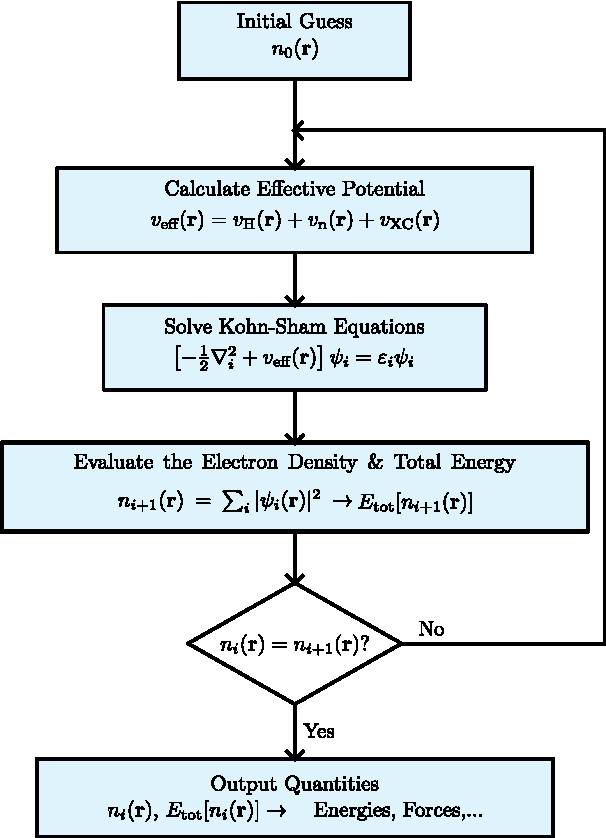
\includegraphics[width=0.6\textwidth]{vasp-workflow.pdf}
    \caption{
        Self-consistent field (SFC) cycle in VASP for DFT calculations adapted from Ref.\supercite{sholl2023density}. The entire cycle starts with an initial guess of the electronic density $n_0(\mathbf{r})$, which then is used to calculate the effective potential $v_{\text{eff}}(\mathbf{r})$. Then, the resulting potential is used to solve the Kohn-Sham equations, from which single-electron wavefunctions $\psi_i(\mathbf{r})$ are obtained. Consequently, the new electronic density $n_{i+1}(\mathbf{r})$ is calculated. Should the old and new densities be close enough---up to a predefined threshold---the cycle stops, and the final electronic density is used to calculate the energies, forces and stress tensor of the system. Otherwise, the cycle repeats itself until convergence is achieved. 
    }
    \label{fig:vasp_workflow}
\end{figure}

\section{VASP Input \& Output Files}
The VASP input and output files are essential for our calculations. On the one hand, the input files contains necessary information---such as the initial structure, exchange-correlation functionals, PAW pseudopotentials, k-point grid, and convergence criteria---that guide the different simulations. On the other hand, the output files contain the results of the different simulations, such as the total enery, forces, stress tensor, and the fully relaxed structure.

This section provides an overview of the required input files for VASP calculations, as well as some relevant output files. For a detailed and rather technical description of the files herein described, we refer the reader to the VASP manual\supercite{zotero-item-672}

\subsection{Input Files}
\subsubsection{INCAR}
The \texttt{INCAR} file defines the computational parameters in VASP and specifies the type of calculation to be performed. Each simulation stage---such as structure optimisation, Density of States (DOS) calculations, AIMD simulations, or MLFF training---are defined by an specific set of INCAR tags. This parameters control convergence thresholds, exchange-correlation functionals, long-range corrections, ensemble choices, and other simulation parameters. If not specified by the user, VASP uses default values. Nonetheless, for reliable and reproducible results, main parameters must be tailored to the system and the type of calculation.


\subsubsection{POSCAR}
The \texttt{POSCAR} (see Figure \ref{fig:csh_poscar}) file provides the actual structure to be studied. It is subdivided into several sections, each one providing specific information about the system.
\begin{figure}[h]
\resizebox{\textwidth}{!}{
\begin{tabular}{>{\columncolor{blue!10}}c>{\columncolor{blue!10}}c>{\columncolor{blue!10}}c
>{\columncolor{blue!10}}l>{\columncolor{blue!10}}l>{\columncolor{blue!10}}l>{\columncolor{blue!10}}l
>{\columncolor{blue!10}}l>{\columncolor{blue!10}}l>{\columncolor{blue!10}}l>{\columncolor{blue!10}}l
>{\columncolor{blue!10}}l>{\columncolor{blue!10}}l>{\columncolor{blue!10}}l>{\columncolor{blue!10}}l
>{\columncolor{blue!10}}l>{\columncolor{blue!10}}l>{\columncolor{blue!10}}l>{\columncolor{blue!10}}l
>{\columncolor{blue!10}}l>{\columncolor{blue!10}}l>{\columncolor{blue!10}}l>{\columncolor{blue!10}}l
>{\columncolor{blue!10}}l>{\columncolor{blue!10}}l}
\hline
\multicolumn{3}{l}{\cellcolor{blue!10} \textbf{Ca Si O H}} & & & & & & & & & & & & & & & & & & & & & & \\
\multicolumn{3}{l}{\cellcolor{blue!10}1.0} & & & & & & & & & & & & & & & & & & & & & & \\
13.18335946 & 0.18445997 & 0.00755401 & & & & & & & & & & & & & & & & & & & & & & \\
-16.45244030 & 24.21622147 & -0.00875423 & & & & & & & & & & & & & & & & & & & & & & \\
1.20664987 & -0.82375620 & 23.18729854 & & & & & & & & & & & & & & & & & & & & & & \\
\multicolumn{3}{l}{\cellcolor{blue!10} \textbf{Ca Si O H}} & & & & & & & & & & & & & & & & & & & & & & \\
\multicolumn{3}{l}{\cellcolor{blue!10}99 60 323 208} & & & & & & & & & & & & & & & & & & & & & & \\
\multicolumn{3}{l}{\cellcolor{blue!10}Direct} & & & & & & & & & & & & & & & & & & & & & & \\
0.38821570 & 0.10613519 & 0.29312228 & & & & & & & & & & & & & & & & & & & & & & \\
0.37259751 & 0.56538816 & 0.26881558 & & & & & & & & & & & & & & & & & & & & & & \\
0.37469040 & 0.31600944 & 0.23882914 & & & & & & & & & & & & & & & & & & & & & & \\
0.35542617 & 0.78384113 & 0.38748504 & & & & & & & & & & & & & & & & & & & & & & \\
0.91347068 & 0.11233954 & 0.31634176 & & & & & & & & & & & & & & & & & & & & & & \\
0.90355777 & 0.57838562 & 0.23567872 & & & & & & & & & & & & & & & & & & & & & & \\
0.87836092 & 0.32109531 & 0.25338100 & & & & & & & & & & & & & & & & & & & & & & \\
0.84529168 & 0.81264469 & 0.29236748 & & & & & & & & & & & & & & & & & & & & & & \\
0.11769176 & 0.02588977 & 0.65372010 & & & & & & & & & & & & & & & & & & & & & & \\
\hline
\end{tabular}
}
\caption{Unit cell structure in fractional coordinates for the \ce{CSH} (Calcium-Silicate-Hydrate) system. The lattice vectors, atomic species (99 Ca, 60 Si, 323 O, 208 H), and the first 9 atomic positions are shown. All coordinates are expressed in direct (fractional) form.}
\label{fig:csh_poscar}
\end{figure}
The first line contains a comment specifying the name of the system or a brief description. Lines 2-4 provide the scaling factor and the corresponding lattice vectors. The actual lattice vectors are obtained by mutiplying the scaling factor (line 2) by the numbers in lines 3-5. Lines 6-7 specify the atomic species as well as the number of ions of each species. Finally, lines 9-onwards provide the ionic positions in angstroms. 

\subsubsection{KPOINTS}
Defining the k-point grid is an essential and one of the first steps when performing DFT calculations, as the accuracy and convergence of the results depend on it. Figure \ref{kpoints} illustrates the \texttt{KPOINTS} file used in this work. The specified mesh is a $1\times 1\times 1$ Gamma centered grid, obtained after a convergence test. 
\begin{figure}[H]
\resizebox{\textwidth}{!}{
	\begin{tabular}{>{\columncolor{blue!10}}c>{\columncolor{blue!10}}l>{\columncolor{blue!10}}l>{\columncolor{blue!10}}l>{\columncolor{blue!10}}l>{\columncolor{blue!10}}l>{\columncolor{blue!10}}l>{\columncolor{blue!10}}l>{\columncolor{blue!10}}l>{\columncolor{blue!10}}l>{\columncolor{blue!10}}l>{\columncolor{blue!10}}l>{\columncolor{blue!10}}l>{\columncolor{blue!10}}l>{\columncolor{blue!10}}l>{\columncolor{blue!10}}l>{\columncolor{blue!10}}l>{\columncolor{blue!10}}l>{\columncolor{blue!10}}l>{\columncolor{blue!10}}l>{\columncolor{blue!10}}l>{\columncolor{blue!10}}l>{\columncolor{blue!10}}l>{\columncolor{blue!10}}l>{\columncolor{blue!10}}l>{\columncolor{blue!10}}l>{\columncolor{blue!10}}l>{\columncolor{blue!10}}l>{\columncolor{blue!10}}l>{\columncolor{blue!10}}l>{\columncolor{blue!10}}l>{\columncolor{blue!10}}l>{\columncolor{blue!10}}l>{\columncolor{blue!10}}l>{\columncolor{blue!10}}l>{\columncolor{blue!10}}l>{\columncolor{blue!10}}l} \hline
		\multicolumn{1}{l}{\cellcolor{blue!10} \textbf{CSH kpoints}} & & & & & & & & & & & & & & & & & & & & & & & & & & & & & & & & & & & &\\ 
		\multicolumn{1}{l}{\cellcolor{blue!10}0}& & & & & & & & & & & & & & & & & & & & & & & & & & & & & & & & & & & &\\
		\multicolumn{1}{l}{\cellcolor{blue!10} \textbf{Gamma}}& & & & & & & & & & & & & & & & & & & & & & & & & & & & & & & & & & & &\\ 
		1 1 1& & & & & & & & & & & & & & & & & & & & & & & & & & & & & & & & & & & & \\
		0 0 0& & & & & & & & & & & & & & & & & & & & & & & & & & & & & & & & & & & & \\  \hline
	\end{tabular}
 }
	\centering
	\caption{CSH k-point grid centerd at the Gamma point. The values "1 1 1" define the grid dimensions in the x, y and z directions. For large systems, a Gamma-centered grid is enough to achieve convergence.}
	\label{kpoints}
\end{figure}

\subsubsection{POTCAR}
The \texttt{POTCAR} file contains the PAW pseudopotentials for each atomic species in the system. As such, it defines how valence electrons interact with the atomic cores. It is constructed by concatenating the individual POTCAR files for each species into a single file. In our work we employed the following PAW pseudopotentials from the PAW\_PBE library:
\begin{itemize}
    \item Ca: Ca\_pv ([Ar] 4s$^2$)
    \item Si: Si ([Ne] 3s$^2$ 3p$^2$)
    \item O: O ([He] 2s$^2$ 2p$^4$)
    \item H: H (1s$^1$)
\end{itemize}

\subsection{Output Files}
These are the main output files generated upon finishing a FP calculation in VASP. They provide essential information about the performance of the calculations, serving as a record of the simulation and allowing for further analysis.
\subsubsection{OUTCAR}
The \texttt{OUTCAR} file is a comprehensive output file that contains detailed information about the VASP calculation. It includes a summary of the input parameters, the evolution of the SCF cycle, the total energy, forces on the atoms, and stress tensor.
\subsubsection{CONTCAR}
The \texttt{CONTCAR} file records the final atomic positions and lattice vectors after a structure relaxation or optimisation. Besides, this file may also contain atomic velocities and predictor-corrector information if written during an AIMD simulation. It has a compatible format with the \texttt{POSCAR} file, making it reausable as an input structure for subsequent calculations.

\subsubsection{DOSCAR}
The \texttt{DOSCAR} file stores the Density of States (DOS) and integrated DOS, expressed in states/eV and cumulative number of states, respectively. This data is especially useful for analysing the electronic properties of the system, and understanding features such as the band gap and the distribution of states across the valence and conduction bands. 
\subsubsection{OSZICAR}
The \texttt{OSZICAR} file records a summary of the electronic and ionic iterations during a DFT calculation. It allows the user to monitor the progress of the SCF cycle convergence, visualise changes in the total energy, and follow the evolution of the ionic relaxation process. 
\subsubsection{ML\_ABN}
The \texttt{ML\_ABN} file contains the training dataset collected during an on-the-fly MLFF training process. As previously described, the MLFF is trained together with an AIMD simulation, where atomic configurations are sampled. Representative configurations are then written to this file, which can be reused to continue the training by renaiming it to a \texttt{ML\_AB} file.

\subsubsection{ML\_FFN}
The \texttt{ML\_FFN} file is a binary file that stores the trained machine learning force field (MLFF) model at the end of the training phase. It contains the model parameters, such as weights and hyperparameters, that define the MLFF. The model can be used for prediction or further refinement by renaming it to an \texttt{ML\_FF} file.


\section{Strucure Relaxation}
Relaxing the CSH structure is a crucial step towards obtaining equilibrium properties of this material. This process involves minimising both the forces on atoms and the total energy of the system, leading to a stable configuration. In this work, we performed the structure relaxation in two stages: an initial relaxation is performed using DFTB+, necessary to obtain a good starting point for VASP and to reduce the computational cost of the full structure relaxation. Thez second stage consists of a full structure relaxation using VASP. Here we outline both stages of the structure relaxation process.

\subsection{Initial Relaxation with DFTB+}
Given the large size of the CSH structure, it was necessary to perform a preliminary relaxation using the GFN1-xTB method implemented in DFTB+. For this step, it was necessary to carry out a k-points convergence test. We then plugged this value into the relaxation script in order to run the structure relaxation. This trick allows us to take our structure closer to its equilibrium configuration, without spending too much time and computational power to do so. This approach is valid as we are not using the final structure as our true optimised structure, but rather as a way to reduce the computation time the full structure relaxation in VASP will take.  

\subsection{Full Structure Relaxation with VASP}
After the rough approximation provided by DFTB+, a full structure relaxation is performed using VASP. To achieve this, we first perform a k-point convergence test, followed by a cut-off energy convergence test. Thereafter, the k-point mesh was defined in the \texttt{KPOINTS} file, and the cut-off energy in the \texttt{INCAR} file where we also specified the PBEsol functional and a force convergence criteria of 0.01 eV/\AA. Once the structure has been fully relaxed, it is used to study the Density of States (DOS) and to train the machine learning force field.

\section{Machine Learning Force Field Generation}
This stage is subdivided into three main phases: training, refinement and testing. In this section we describe each one of them in detail 
\subsection{Training}
As previously disscused, the MLFF is generated on-the-fly during a AIMD simulation. To begin, we use the \texttt{CONTCAR} file containing our relaxed structure as the input \texttt{POSCAR} file for this step. In the \texttt{INCAR} file some parameters need to be set: \texttt{IBRION=0}, indicates VASP to switch to an AIMD simulation; \texttt{NSW=50000} indicates the number of ionic steps; \texttt{POTIM=2.0} is the MD time step in fs; \texttt{MDALGO=3} tells VASP to use the Langevin thermostat; \texttt{TEBEG=400} sets the temperature (in K) at wich the simulation is performed, and \texttt{ISIF=3} allows for positions, cell shape and volume to be updated. 

Finally, \texttt{ML\_LMLFF=T} and \texttt{ML\_ISTART=0} tags govern the MLFF training process. The former enables the use of machine learning force fields, and the latter tells VASP to generate a new MLFF from scratch. Even though, the parameters herein described are the most important, additional tags may need to be set depending on the performance of the training phase

\subsection{Refinement}
The refinement phase allows for improvements to be made in the generated MLFF model by tunning the hyperparameters in the model. To this end, we first need to 

\subsection{Testing}


\chapter{Results \& Discussion}
\label{Chapter4}
\lhead{Chapter 4. \emph{Results \& Discussion}}

\section{My results}
Hello
\begin{figure}[H]
    \centering
    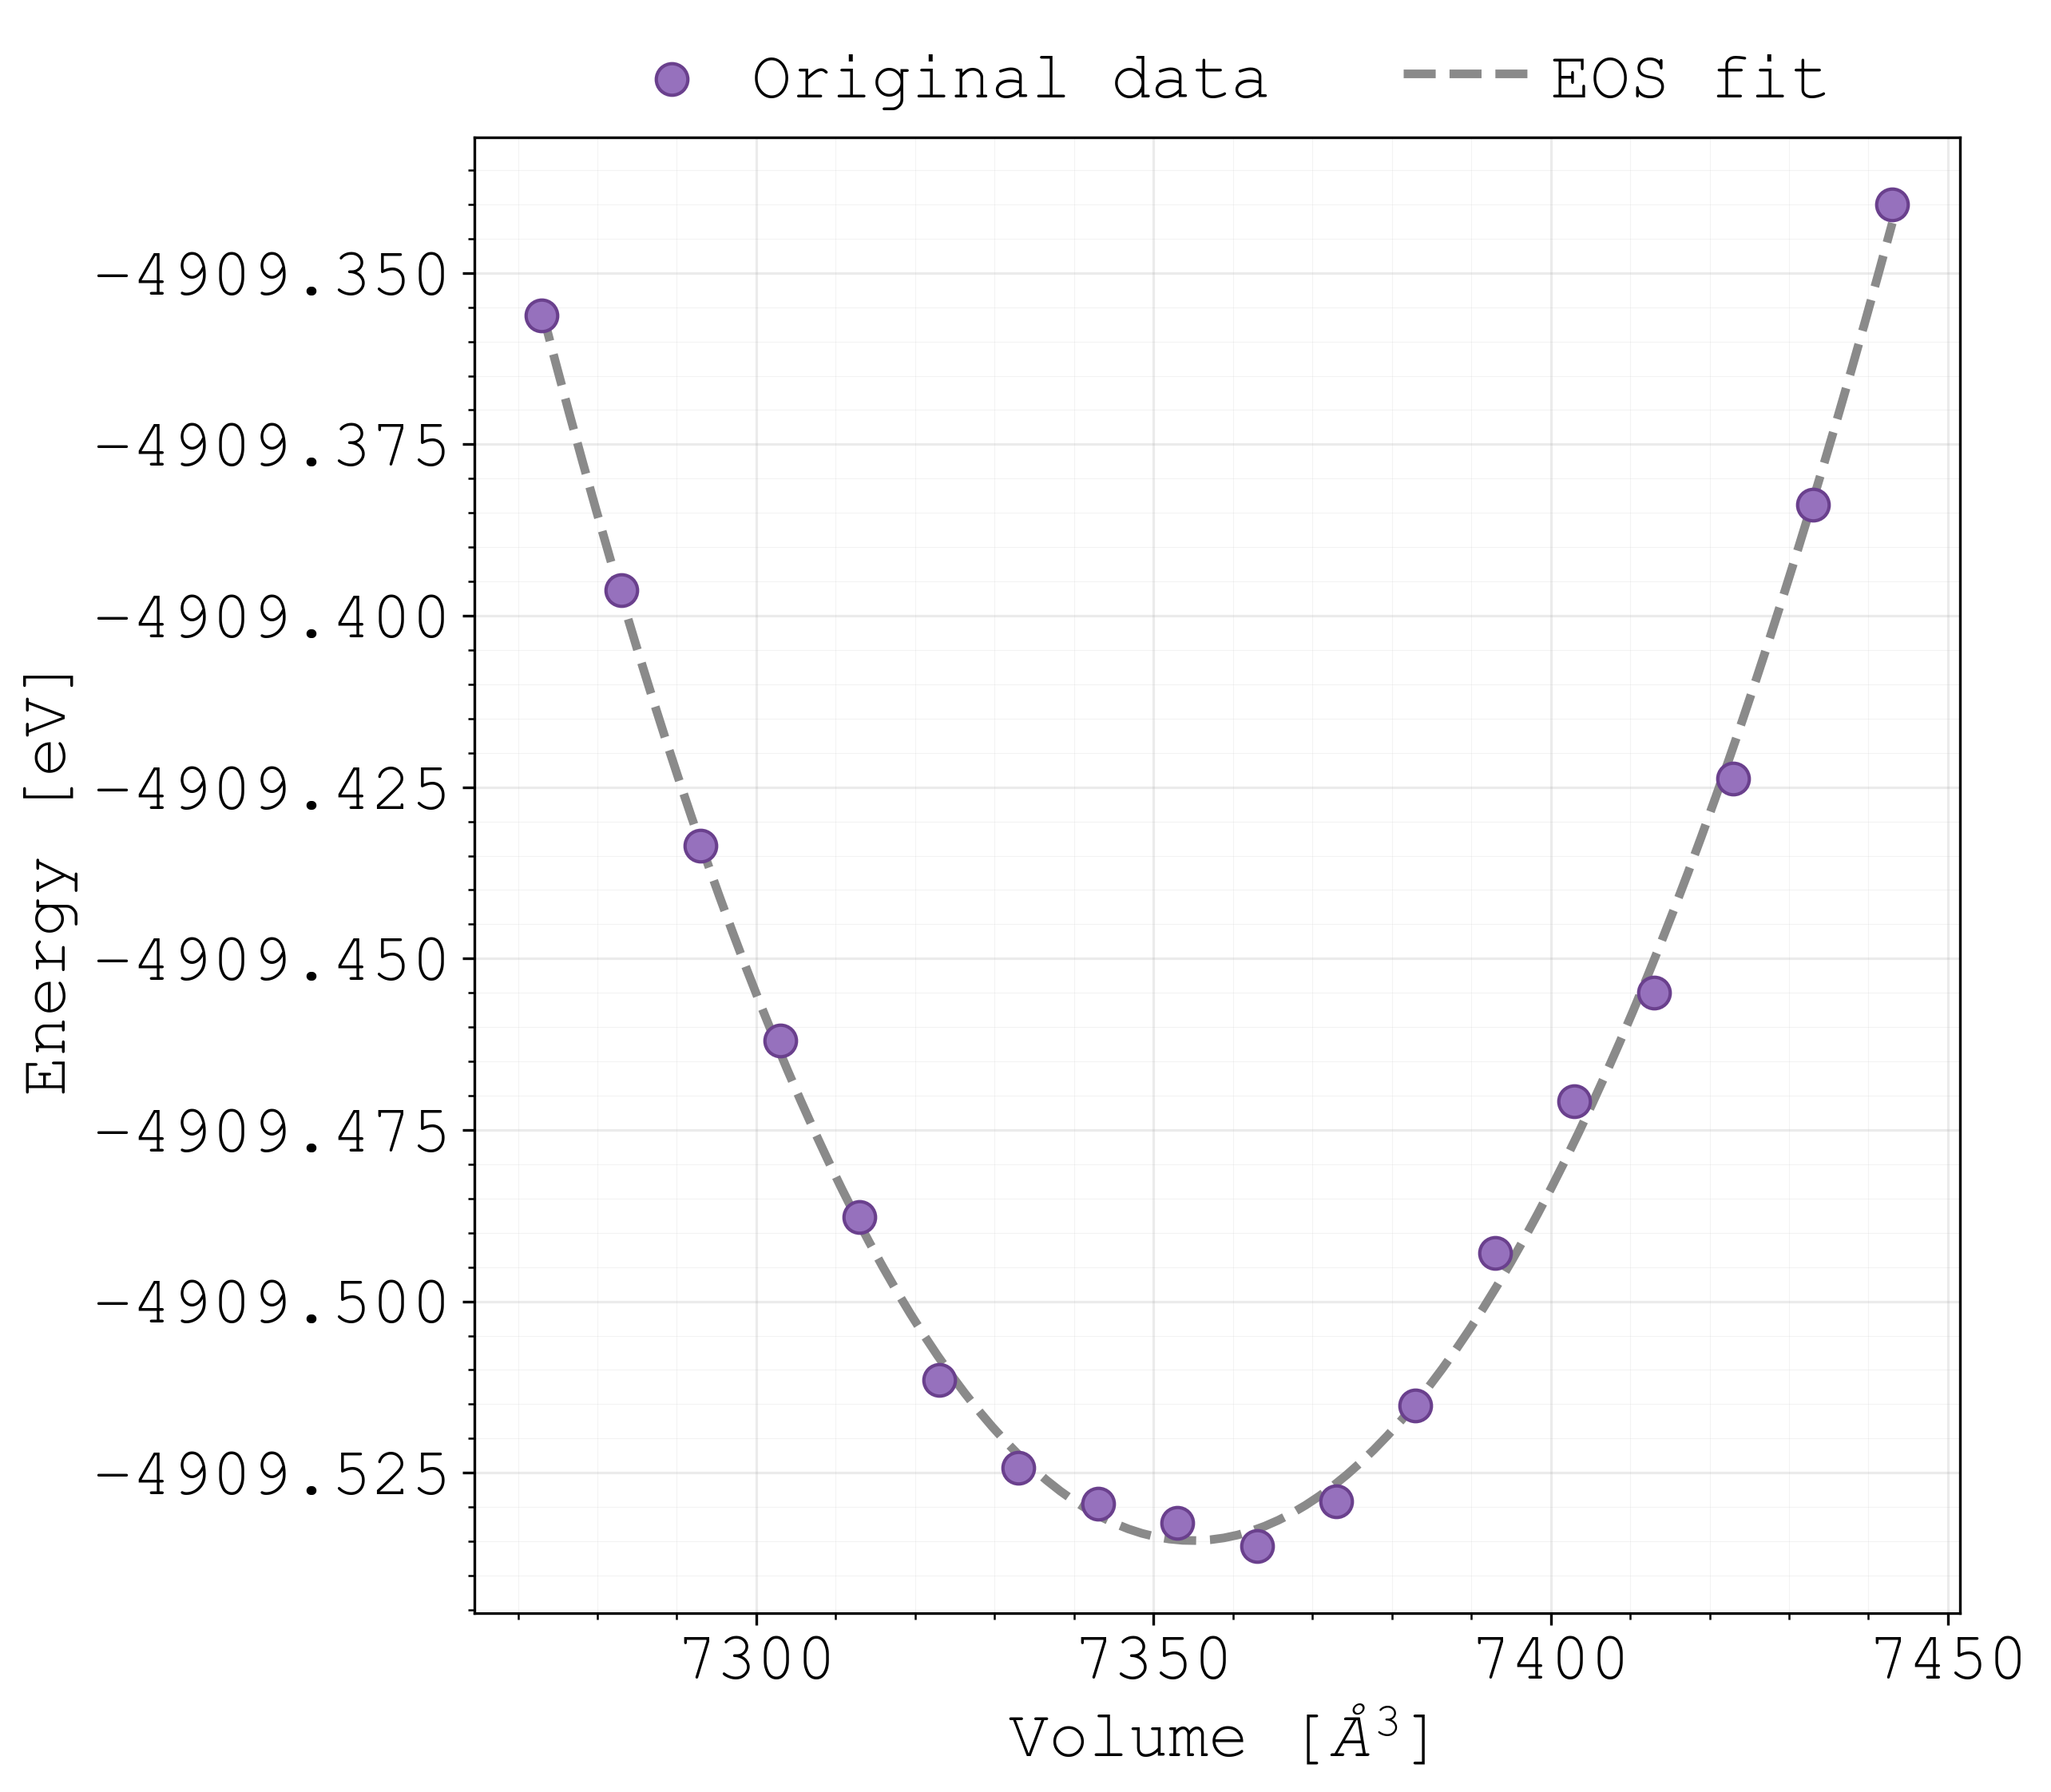
\includegraphics[width=0.5\textwidth]{EOS_SA_EDIFF_02.png}
    \caption{A schematic representation of the DFT formalism. The many-body wavefunction is replaced by a single-particle wavefunction, which is used to calculate the electron density. The electron density is then used to calculate the total energy of the system. Adapted from \supercite{giustino2014materials}.}
    \label{fig:dft}
\end{figure}

%% Chapter 5
\chapter{\texorpdfstring{Conclusions $\&$ Outlook}{Conclusions \& Outlook}} % Main chapter title

\label{Chapter5} % For referencing the chapter elsewhere, use \ref{Chapter5}

\lhead{Chapter 5. \emph{Conclusions $\&$ Outlook}} % This is for the header on each page - perhaps a shortened title

This work provides a comprehensive analysis of the magnetic and electronic properties of XGeTe$_3$ (X = Cr, Mn, Fe) monolayers and their random alloys, including Cr$_{1-x}$GeMn$_{x}$Te$_3$, Cr$_{1-x}$GeFe$_{x}$Te$_3$, and Fe$_{1-x}$GeMn$_{x}$Te$_3$, using density functional theory (DFT) with PBE and PBESol functionals, alongside Hubbard $U$ corrections.

For the CrGeTe$_3$ monolayer, we confirmed robust ferromagnetic (FM) ordering, driven by strong exchange interactions. The PBE+U functional, with $U = 3.0$ eV, offered a balanced trade-off between computational efficiency and accuracy. The calculated band gap aligned well with experimental data. Phonon stability analysis confirmed the dynamical stability of the system, supporting its potential for practical applications. Future studies may benefit from using more advanced functionals for deeper exploration of its electronic and magnetic properties.

The MnGeTe$_3$ monolayer exhibited half-metallic (HM) behavior, making it suitable for spintronic applications. The PBE+U functional, with $U = 2.5$ eV, effectively captured both the magnetic moments and ground state energies. Phonon analysis confirmed its dynamical stability, positioning MnGeTe$_3$ as a promising material for further refinement of the Hubbard $U$ parameter or exploration of alternative functionals.

The FeGeTe$_3$ monolayer displayed distinct deviations from the symmetrical behavior observed in CrGeTe$_3$ and MnGeTe$_3$. These deviations were attributed to its antiferromagnetic (AFM) ground state and the hybridization between Fe $d$ states and Te $p$ states. Phonon analysis revealed negative frequencies, suggesting potential dynamical instabilities that need to be addressed to fully understand and optimize the electronic properties of FeGeTe$_3$.

For the random alloys, substitution of Cr, Mn, and Fe atoms in XGeTe$_3$ supercells led to notable changes in magnetic moments, electronic structures, and alloy stability. In Cr$_{1-x}$GeMn$_{x}$Te$_3$ at $x = 0.50$, magnetic moment disorder was observed, where one Mn atom exhibited a negative magnetic moment due to local atomic environments and magnetic frustration linked to variations in Mn-Te bond lengths. This suggests the presence of complex magnetic ground states, which could be beneficial for spintronic applications. Negative formation energies across different concentrations confirmed the alloy's global thermodynamic stability, while positive mixing energies indicated structural complexity that could give rise to non-ferromagnetic phases.

In Cr$_{1-x}$GeFe$_{x}$Te$_3$, at $x = 0.75$, strong hybridization between Fe and Cr $d$ states and Te $p$ states was observed, indicating the tunability of electronic transport properties through Fe doping. This positions the alloy as a promising candidate for applications in magnetic sensors and thermoelectric devices. The consistent magnetic moments and stable formation energies across concentrations further affirm its technological viability.

In the Fe$_{1-x}$GeMn$_{x}$Te$_3$ system, increasing Mn concentrations (up to $x = 0.75$) led to structural tension and strong hybridization between Mn and Fe $d$ states with Te. This suggests the alloy’s potential for applications in magnetic tunneling junctions and other devices requiring tailored electronic and magnetic properties. However, despite the negative formation energies confirming thermodynamic stability, the structural tensions at high Mn concentrations must be addressed to fully harness the alloy's technological potential.

In conclusion, this investigation underscores the significant technological potential of XGeTe$_3$ monolayers and their random alloys for applications in spintronics, magnetic memory, and thermoelectric devices. Precise control over magnetic frustration, hybridization, and alloy stability is essential for the successful deployment of these materials, paving the way for future research in this rapidly advancing field.
%\input{Chapters/Chapter6}
% \input{Chapters/Chapter7}

%-------------------------------------------------------------------------------
%	THESIS CONTENT - APPENDICES
%-------------------------------------------------------------------------------

\addtocontents{toc}{\vspace{2em}} % Add a gap in the Contents, for aesthetics

\appendix % Cue to tell LaTeX that the following 'chapters' are Appendices

% Include the appendices of the thesis as separate files from the Appendices
% folder
% Uncomment the lines as you write the Appendices

%\chapter{Appendix A} % Main appendix title
\vspace{-2.5cm}
%\label{Appendix} % Change X to a consecutive letter; this is for the header on each page - perhaps a shortened title
\begin{figure}[H]
\centering
\begin{subfigure}{0.24\textwidth}
    \centering
    \includegraphics[width=\textwidth]{Figures/Appendix/CGT/PBE/dosplot_Cr_pbe.png}
    \label{dosplot_Cr_pbe}
\end{subfigure}
\hfill
\begin{subfigure}{0.24\textwidth}
\centering
    \includegraphics[width=\textwidth]{Figures/Appendix/CGT/PBE/dosplot_Crs_pbe.png}
    \label{dosplot_Crs_pbe}
\end{subfigure}
\hfill
\begin{subfigure}{0.24\textwidth}
    \includegraphics[width=\textwidth]{Figures/Appendix/CGT/PBE/dosplot_Crd_pbe.png}
    \label{dosplot_Crd_pbe}
\end{subfigure}
\hfill
\begin{subfigure}{0.24\textwidth}
    \includegraphics[width=\textwidth]{Figures/Appendix/CGT/PBE/dosplot_Crdx2_pbe.png}
    \label{dodosplot_Crdx2_pbe}
\end{subfigure}
\hfill
\begin{subfigure}{0.24\textwidth}
    \includegraphics[width=\textwidth]{Figures/Appendix/CGT/PBE/dosplot_Crdxy_pbe.png}
    \label{dosplot_Crdxy_pbe}
\end{subfigure}
\hfill
\begin{subfigure}{0.24\textwidth}
    \includegraphics[width=\textwidth]{Figures/Appendix/CGT/PBE/dosplot_Crdxz_pbe.png}
    \label{dosplot_Crdxz_pbe}
\end{subfigure}
\hfill
\begin{subfigure}{0.24\textwidth}
    \includegraphics[width=\textwidth]{Figures/Appendix/CGT/PBE/dosplot_Crdyz_pbe.png}
    \label{dosplot_Crdyz_pbe}
\end{subfigure}
\hfill
\begin{subfigure}{0.24\textwidth}
    \includegraphics[width=\textwidth]{Figures/Appendix/CGT/PBE/dosplot_Crdz2_pbe.png}
    \label{dosplot_Crdz2_pbe}
\end{subfigure}
\hfill
\begin{subfigure}{0.24\textwidth}
    \includegraphics[width=\textwidth]{Figures/Appendix/CGT/PBE/dosplot_Crt2g_pbe.png}
    \label{dosplot_Crt2g_pbe}
\end{subfigure}
\hfill
\begin{subfigure}{0.24\textwidth}
    \includegraphics[width=\textwidth]{Figures/Appendix/CGT/PBE/dosplot_Creg_pbe.png}
    \label{dosplot_Creg_pbe}
\end{subfigure}
\hfill
\begin{subfigure}{0.24\textwidth}
    \includegraphics[width=\textwidth]{Figures/Appendix/CGT/PBE/dosplot_Ge_pbe.png}
    \label{dosplot_Ge_pbe}
\end{subfigure}
\hfill
\begin{subfigure}{0.24\textwidth}
    \includegraphics[width=\textwidth]{Figures/Appendix/CGT/PBE/dosplot_Ges_pbe.png}
    \label{dosplot_Ges_pbe}
\end{subfigure}
\hfill
\begin{subfigure}{0.24\textwidth}
    \includegraphics[width=\textwidth]{Figures/Appendix/CGT/PBE/dosplot_Gep_pbe.png}
    \label{dosplot_Gep_pbe}
\end{subfigure}
\hfill
\begin{subfigure}{0.24\textwidth}
    \includegraphics[width=\textwidth]{Figures/Appendix/CGT/PBE/dosplot_Gepx_pbe.png}
    \label{dosplot_Gepx_pbe}
\end{subfigure}
\hfill
\begin{subfigure}{0.24\textwidth}
    \includegraphics[width=\textwidth]{Figures/Appendix/CGT/PBE/dosplot_Gepy_pbe.png}
    \label{dosplot_Gepy_pbe}
\end{subfigure}
\hfill
\begin{subfigure}{0.24\textwidth}
    \includegraphics[width=\textwidth]{Figures/Appendix/CGT/PBE/dosplot_Gepz_pbe.png}
    \label{dosplot_Gepz_pbe}
\end{subfigure}
\hfill
\begin{subfigure}{0.24\textwidth}
    \includegraphics[width=\textwidth]{Figures/Appendix/CGT/PBE/dosplot_Te_pbe.png}
    \label{dosplot_Te_pbe}
\end{subfigure}
\hfill
\begin{subfigure}{0.24\textwidth}
    \includegraphics[width=\textwidth]{Figures/Appendix/CGT/PBE/dosplot_Tes_pbe.png}
    \label{dosplot_Tes_pbe}
\end{subfigure}
\hfill
\begin{subfigure}{0.24\textwidth}
    \includegraphics[width=\textwidth]{Figures/Appendix/CGT/PBE/dosplot_Tep_pbe.png}
    \label{dosplot_Tep_pbe}
\end{subfigure}
\hfill
\begin{subfigure}{0.24\textwidth}
    \includegraphics[width=\textwidth]{Figures/Appendix/CGT/PBE/dosplot_Tepx_pbe.png}
    \label{dosplot_Tepx_pbe}
\end{subfigure}
\hfill
\begin{subfigure}{0.24\textwidth}
    \includegraphics[width=\textwidth]{Figures/Appendix/CGT/PBE/dosplot_Tepy_pbe.png}
    \label{dosplot_Tepy_pbe}
\end{subfigure}
\begin{subfigure}{0.24\textwidth}
    \includegraphics[width=\textwidth]{Figures/Appendix/CGT/PBE/dosplot_Tepz_pbe.png}
    \label{dosplot_Tepz_pbe}
\end{subfigure}
\hfill
\caption{Detailed density of states for the ferromagnetic CrGeTe$_3$ monolayer, calculated using the PBE functional for each atomic orbital, is shown. The horizontal axis represents the energy difference $E - E_F$, while the vertical axis indicates the normalized density of states (states/eV).}
\label{Crpbe}
\end{figure}


%--------------------------------------------------------------------------------------------
\newpage
 \begin{figure}[H]
      \centering
    \begin{subfigure}{0.24\textwidth}
    \includegraphics[width=\textwidth]{Figures/Appendix/CGT/PBESol/dosplot_Cr_pbesol.png}
    \label{dosplot_Cr_pbesol}   
    \end{subfigure}  
    \hfill
\begin{subfigure}{0.24\textwidth}
\centering
    \includegraphics[width=\textwidth]{Figures/Appendix/CGT/PBESol/dosplot_Crs_pbesol.png}
    \label{dosplot_Crs_pbesol}
\end{subfigure}
\hfill
\begin{subfigure}{0.24\textwidth}
    \includegraphics[width=\textwidth]{Figures/Appendix/CGT/PBESol/dosplot_Crd_pbesol.png}
    \label{dosplot_Crd_pbesol}
\end{subfigure}
\hfill
\begin{subfigure}{0.24\textwidth}
    \includegraphics[width=\textwidth]{Figures/Appendix/CGT/PBESol/dosplot_Crdx2_pbesol.png}
    \label{dodosplot_Crdx2_pbesol}
\end{subfigure}
\hfill
\begin{subfigure}{0.24\textwidth}
    \includegraphics[width=\textwidth]{Figures/Appendix/CGT/PBESol/dosplot_Crdxy_pbesol.png}
    \label{dosplot_Crdxy_pbesol}
\end{subfigure}
\hfill
\begin{subfigure}{0.24\textwidth}
    \includegraphics[width=\textwidth]{Figures/Appendix/CGT/PBESol/dosplot_Crdxz_pbesol.png}
    \label{dosplot_Crdxz_pbesol}
\end{subfigure}
\hfill
\begin{subfigure}{0.24\textwidth}
    \includegraphics[width=\textwidth]{Figures/Appendix/CGT/PBESol/dosplot_Crdyz_pbesol.png}
    \label{dosplot_Crdyz_pbesol}
\end{subfigure}
\hfill
\begin{subfigure}{0.24\textwidth}
    \includegraphics[width=\textwidth]{Figures/Appendix/CGT/PBESol/dosplot_Crdz2_pbesol.png}
    \label{dosplot_Crdz2_pbesol}
\end{subfigure}
\hfill
\begin{subfigure}{0.24\textwidth}
    \includegraphics[width=\textwidth]{Figures/Appendix/CGT/PBESol/dosplot_Crt2g_pbesol.png}
    \label{dosplot_Crt2g_pbesol}
\end{subfigure}
\hfill
\begin{subfigure}{0.24\textwidth}
    \includegraphics[width=\textwidth]{Figures/Appendix/CGT/PBESol/dosplot_Creg_pbesol.png}
    \label{dosplot_Creg_pbesol}
\end{subfigure}
\hfill
\begin{subfigure}{0.24\textwidth}
    \includegraphics[width=\textwidth]{Figures/Appendix/CGT/PBESol/dosplot_Ge_pbesol.png}
    \label{dosplot_Ge_pbesol}
\end{subfigure}
\hfill
\begin{subfigure}{0.24\textwidth}
    \includegraphics[width=\textwidth]{Figures/Appendix/CGT/PBESol/dosplot_Ges_pbesol.png}
    \label{dosplot_Ges_pbesol}
\end{subfigure}
\hfill
\begin{subfigure}{0.24\textwidth}
    \includegraphics[width=\textwidth]{Figures/Appendix/CGT/PBESol/dosplot_Gep_pbesol.png}
    \label{dosplot_Gep_pbesol}
\end{subfigure}
\hfill
\begin{subfigure}{0.24\textwidth}
    \includegraphics[width=\textwidth]{Figures/Appendix/CGT/PBESol/dosplot_Gepx_pbesol.png}
    \label{dosplot_Gepx_pbesol}
\end{subfigure}
\hfill
\begin{subfigure}{0.24\textwidth}
    \includegraphics[width=\textwidth]{Figures/Appendix/CGT/PBESol/dosplot_Gepy_pbesol.png}
    \label{dosplot_Gepy_pbesol}
\end{subfigure}
\hfill
\begin{subfigure}{0.24\textwidth}
    \includegraphics[width=\textwidth]{Figures/Appendix/CGT/PBESol/dosplot_Gepz_pbesol.png}
    \label{dosplot_Gepz_pbesol}
\end{subfigure}
\hfill
\begin{subfigure}{0.24\textwidth}
    \includegraphics[width=\textwidth]{Figures/Appendix/CGT/PBESol/dosplot_Te_pbesol.png}
    \label{dosplot_Te_pbesol}
\end{subfigure}
\hfill
\begin{subfigure}{0.24\textwidth}
    \includegraphics[width=\textwidth]{Figures/Appendix/CGT/PBESol/dosplot_Tes_pbesol.png}
    \label{dosplot_Tes_pbesol}
\end{subfigure}
\hfill
\begin{subfigure}{0.24\textwidth}
    \includegraphics[width=\textwidth]{Figures/Appendix/CGT/PBESol/dosplot_Tep_pbesol.png}
    \label{dosplot_Tep_pbesol}
\end{subfigure}
\hfill
\begin{subfigure}{0.24\textwidth}
    \includegraphics[width=\textwidth]{Figures/Appendix/CGT/PBESol/dosplot_Tepx_pbesol.png}
    \label{dosplot_Tepx_pbesol}
\end{subfigure}
\hfill
\begin{subfigure}{0.24\textwidth}
    \includegraphics[width=\textwidth]{Figures/Appendix/CGT/PBESol/dosplot_Tepy_pbesol.png}
    \label{dosplot_Tepy_pbesol}
\end{subfigure}
\begin{subfigure}{0.24\textwidth}
    \includegraphics[width=\textwidth]{Figures/Appendix/CGT/PBESol/dosplot_Tepz_pbesol.png}
    \label{dosplot_Tepz_pbesol}
\end{subfigure}
\hfill
     \caption{Detailed density of states for the ferromagnetic CrGeTe$_3$ monolayer, calculated using the PBESol functional for each atomic orbital, is shown. The horizontal axis represents the energy difference $E - E_F$, while the vertical axis indicates the normalized density of states (states/eV)}
     \label{CrPbesol}
 \end{figure}

%-----------------------------------------------------------------------------------------------
\newpage
 \begin{figure}[H]
      \centering
    \begin{subfigure}{0.24\textwidth}
    \includegraphics[width=\textwidth]{Figures/Appendix/CGT/HSE06/dosplot_Cr_hse06.png}
    \label{dosplot_Cr_hse06}   
    \end{subfigure}  
    \hfill
\begin{subfigure}{0.24\textwidth}
\centering
    \includegraphics[width=\textwidth]{Figures/Appendix/CGT/HSE06/dosplot_Crs_hse06.png}
    \label{dosplot_Crs_hse06}
\end{subfigure}
\hfill
\begin{subfigure}{0.24\textwidth}
    \includegraphics[width=\textwidth]{Figures/Appendix/CGT/HSE06/dosplot_Crd_hse06.png}
    \label{dosplot_Crd_hse06}
\end{subfigure}
\hfill
\begin{subfigure}{0.24\textwidth}
    \includegraphics[width=\textwidth]{Figures/Appendix/CGT/HSE06/dosplot_Crdx2_hse06.png}
    \label{dodosplot_Crdx2_hse06}
\end{subfigure}
\hfill
\begin{subfigure}{0.24\textwidth}
    \includegraphics[width=\textwidth]{Figures/Appendix/CGT/HSE06/dosplot_Crdxy_hse06.png}
    \label{dosplot_Crdxy_hse06}
\end{subfigure}
\hfill
\begin{subfigure}{0.24\textwidth}
    \includegraphics[width=\textwidth]{Figures/Appendix/CGT/HSE06/dosplot_Crdxz_hse06.png}
    \label{dosplot_Crdxz_hse06}
\end{subfigure}
\hfill
\begin{subfigure}{0.24\textwidth}
    \includegraphics[width=\textwidth]{Figures/Appendix/CGT/HSE06/dosplot_Crdyz_hse06.png}
    \label{dosplot_Crdyz_hse06}
\end{subfigure}
\hfill
\begin{subfigure}{0.24\textwidth}
    \includegraphics[width=\textwidth]{Figures/Appendix/CGT/HSE06/dosplot_Crdz2_hse06.png}
    \label{dosplot_Crdz2_hse06}
\end{subfigure}
\hfill
\begin{subfigure}{0.24\textwidth}
    \includegraphics[width=\textwidth]{Figures/Appendix/CGT/HSE06/dosplot_Crt2g_hse06.png}
    \label{dosplot_Crt2g_hse06}
\end{subfigure}
\hfill
\begin{subfigure}{0.24\textwidth}
    \includegraphics[width=\textwidth]{Figures/Appendix/CGT/HSE06/dosplot_Creg_hse06.png}
    \label{dosplot_Creg_hse06}
\end{subfigure}
\hfill
\begin{subfigure}{0.24\textwidth}
    \includegraphics[width=\textwidth]{Figures/Appendix/CGT/HSE06/dosplot_Ge_hse06.png}
    \label{dosplot_Ge_hse06}
\end{subfigure}
\hfill
\begin{subfigure}{0.24\textwidth}
    \includegraphics[width=\textwidth]{Figures/Appendix/CGT/HSE06/dosplot_Ges_hse06.png}
    \label{dosplot_Ges_hse06}
\end{subfigure}
\hfill
\begin{subfigure}{0.24\textwidth}
    \includegraphics[width=\textwidth]{Figures/Appendix/CGT/HSE06/dosplot_Gep_hse06.png}
    \label{dosplot_Gep_hse06}
\end{subfigure}
\hfill
\begin{subfigure}{0.24\textwidth}
    \includegraphics[width=\textwidth]{Figures/Appendix/CGT/HSE06/dosplot_Gepx_hse06.png}
    \label{dosplot_Gepx_hse06}
\end{subfigure}
\hfill
\begin{subfigure}{0.24\textwidth}
    \includegraphics[width=\textwidth]{Figures/Appendix/CGT/HSE06/dosplot_Gepy_hse06.png}
    \label{dosplot_Gepy_hse06}
\end{subfigure}
\hfill
\begin{subfigure}{0.24\textwidth}
    \includegraphics[width=\textwidth]{Figures/Appendix/CGT/HSE06/dosplot_Gepz_hse06.png}
    \label{dosplot_Gepz_hse06}
\end{subfigure}
\hfill
\begin{subfigure}{0.24\textwidth}
    \includegraphics[width=\textwidth]{Figures/Appendix/CGT/HSE06/dosplot_Te_hse06.png}
    \label{dosplot_Te_hse06}
\end{subfigure}
\hfill
\begin{subfigure}{0.24\textwidth}
    \includegraphics[width=\textwidth]{Figures/Appendix/CGT/HSE06/dosplot_Tes_hse06.png}
    \label{dosplot_Tes_hse06}
\end{subfigure}
\hfill
\begin{subfigure}{0.24\textwidth}
    \includegraphics[width=\textwidth]{Figures/Appendix/CGT/HSE06/dosplot_Tep_hse06.png}
    \label{dosplot_Tep_hse06}
\end{subfigure}
\hfill
\begin{subfigure}{0.24\textwidth}
    \includegraphics[width=\textwidth]{Figures/Appendix/CGT/HSE06/dosplot_Tepx_hse06.png}
    \label{dosplot_Tepx_hse06}
\end{subfigure}
\hfill
\begin{subfigure}{0.24\textwidth}
    \includegraphics[width=\textwidth]{Figures/Appendix/CGT/HSE06/dosplot_Tepy_hse06.png}
    \label{dosplot_Tepy_hse06}
\end{subfigure}
\begin{subfigure}{0.24\textwidth}
    \includegraphics[width=\textwidth]{Figures/Appendix/CGT/HSE06/dosplot_Tepz_hse06.png}
    \label{dosplot_Tepz_hse06}
\end{subfigure}
\hfill
     \caption{Detailed density of states for the ferromagnetic CrGeTe$_3$ monolayer, calculated using the hybrid functional HSE06 for each atomic orbital, is shown. The horizontal axis represents the energy difference $E - E_F$, while the vertical axis indicates the normalized density of states (states/eV)}
     \label{Crhse06}
 \end{figure}

%-----------------------------------------------------------------------------------------------
\newpage
\begin{figure}[H]
\centering
\begin{subfigure}{0.24\textwidth}
    \centering
    \includegraphics[width=\textwidth]{Figures/Appendix/MGT/PBE/dosplot_Mn_pbe.png}
    \label{dosplot_Mn_pbe}
\end{subfigure}
\hfill
\begin{subfigure}{0.24\textwidth}
\centering
    \includegraphics[width=\textwidth]{Figures/Appendix/MGT/PBE/dosplot_Mns_pbe.png}
    \label{dosplot_Mns_pbe}
\end{subfigure}
\hfill
\begin{subfigure}{0.24\textwidth}
    \includegraphics[width=\textwidth]{Figures/Appendix/MGT/PBE/dosplot_Mnd_pbe.png}
    \label{dosplot_Mnd_pbe}
\end{subfigure}
\hfill
\begin{subfigure}{0.24\textwidth}
    \includegraphics[width=\textwidth]{Figures/Appendix/MGT/PBE/dosplot_Mndx2_pbe.png}
    \label{dodosplot_Mndx2_pbe}
\end{subfigure}
\hfill
\begin{subfigure}{0.24\textwidth}
    \includegraphics[width=\textwidth]{Figures/Appendix/MGT/PBE/dosplot_Mndxy_pbe.png}
    \label{dosplot_Mndxy_pbe}
\end{subfigure}
\hfill
\begin{subfigure}{0.24\textwidth}
    \includegraphics[width=\textwidth]{Figures/Appendix/MGT/PBE/dosplot_Mndxz_pbe.png}
    \label{dosplot_Mndxz_pbe}
\end{subfigure}
\hfill
\begin{subfigure}{0.24\textwidth}
    \includegraphics[width=\textwidth]{Figures/Appendix/MGT/PBE/dosplot_Mndyz_pbe.png}
    \label{dosplot_Mndyz_pbe}
\end{subfigure}
\hfill
\begin{subfigure}{0.24\textwidth}
    \includegraphics[width=\textwidth]{Figures/Appendix/MGT/PBE/dosplot_Mndz2_pbe.png}
    \label{dosplot_Mndz2_pbe}
\end{subfigure}
\hfill
\begin{subfigure}{0.24\textwidth}
    \includegraphics[width=\textwidth]{Figures/Appendix/MGT/PBE/dosplot_Mnt2g_pbe.png}
    \label{dosplot_Mnt2g_pbe}
\end{subfigure}
\hfill
\begin{subfigure}{0.24\textwidth}
    \includegraphics[width=\textwidth]{Figures/Appendix/MGT/PBE/dosplot_Mneg_pbe.png}
    \label{dosplot_Mneg_pbe}
\end{subfigure}
\hfill
\begin{subfigure}{0.24\textwidth}
    \includegraphics[width=\textwidth]{Figures/Appendix/MGT/PBE/dosplot_Ge_pbe.png}
    \label{dosplot_MnGe_pbe}
\end{subfigure}
\hfill
\begin{subfigure}{0.24\textwidth}
    \includegraphics[width=\textwidth]{Figures/Appendix/MGT/PBE/dosplot_Ges_pbe.png}
    \label{dosplot_MnGes_pbe}
\end{subfigure}
\hfill
\begin{subfigure}{0.24\textwidth}
    \includegraphics[width=\textwidth]{Figures/Appendix/MGT/PBE/dosplot_Gep_pbe.png}
    \label{dosplot_MnGep_pbe}
\end{subfigure}
\hfill
\begin{subfigure}{0.24\textwidth}
    \includegraphics[width=\textwidth]{Figures/Appendix/MGT/PBE/dosplot_Gepx_pbe.png}
    \label{dosplot_MnGepx_pbe}
\end{subfigure}
\hfill
\begin{subfigure}{0.24\textwidth}
    \includegraphics[width=\textwidth]{Figures/Appendix/MGT/PBE/dosplot_Gepy_pbe.png}
    \label{dosplot_MnGepy_pbe}
\end{subfigure}
\hfill
\begin{subfigure}{0.24\textwidth}
    \includegraphics[width=\textwidth]{Figures/Appendix/MGT/PBE/dosplot_Gepz_pbe.png}
    \label{dosplot_MnGepz_pbe}
\end{subfigure}
\hfill
\begin{subfigure}{0.24\textwidth}
    \includegraphics[width=\textwidth]{Figures/Appendix/MGT/PBE/dosplot_Te_pbe.png}
    \label{dosplot_MnTe_pbe}
\end{subfigure}
\hfill
\begin{subfigure}{0.24\textwidth}
    \includegraphics[width=\textwidth]{Figures/Appendix/MGT/PBE/dosplot_Tes_pbe.png}
    \label{dosplot_MnTes_pbe}
\end{subfigure}
\hfill
\begin{subfigure}{0.24\textwidth}
    \includegraphics[width=\textwidth]{Figures/Appendix/CGT/PBE/dosplot_Tep_pbe.png}
    \label{dosplot_MnTep_pbe}
\end{subfigure}
\hfill
\begin{subfigure}{0.24\textwidth}
    \includegraphics[width=\textwidth]{Figures/Appendix/MGT/PBE/dosplot_Tepx_pbe.png}
    \label{dosplot_MnTepx_pbe}
\end{subfigure}
\hfill
\begin{subfigure}{0.24\textwidth}
    \includegraphics[width=\textwidth]{Figures/Appendix/MGT/PBE/dosplot_Tepy_pbe.png}
    \label{dosplot_MnTepy_pbe}
\end{subfigure}
\begin{subfigure}{0.24\textwidth}
    \includegraphics[width=\textwidth]{Figures/Appendix/MGT/PBE/dosplot_Tepz_pbe.png}
    \label{dosplot_MnTepz_pbe}
\end{subfigure}
\hfill

\caption{Detailed density of states for the ferromagnetic MnGeTe$_3$ monolayer, calculated using the PBE functional for each atomic orbital, is shown. The horizontal axis represents the energy difference $E - E_F$, while the vertical axis indicates the normalized density of states (states/eV)}
\label{Mnpbe}
\end{figure}
%--------------------------------------------------------------------------------------------
\newpage
 \begin{figure}[H]
      \centering
    \begin{subfigure}{0.24\textwidth}
    \includegraphics[width=\textwidth]{Figures/Appendix/MGT/PBESol/dosplot_Mn_pbesol.png}
    \label{dosplot_Mn_pbesol}   
    \end{subfigure}  
    \hfill
\begin{subfigure}{0.24\textwidth}
\centering
    \includegraphics[width=\textwidth]{Figures/Appendix/MGT/PBESol/dosplot_Mns_pbesol.png}
    \label{dosplot_Mns_pbesol}
\end{subfigure}
\hfill
\begin{subfigure}{0.24\textwidth}
    \includegraphics[width=\textwidth]{Figures/Appendix/MGT/PBESol/dosplot_Mnd_pbesol.png}
    \label{dosplot_Mnd_pbesol}
\end{subfigure}
\hfill
\begin{subfigure}{0.24\textwidth}
    \includegraphics[width=\textwidth]{Figures/Appendix/MGT/PBESol/dosplot_Mndx2_pbesol.png}
    \label{dodosplot_Mndx2_pbesol}
\end{subfigure}
\hfill
\begin{subfigure}{0.24\textwidth}
    \includegraphics[width=\textwidth]{Figures/Appendix/MGT/PBESol/dosplot_Mndxy_pbesol.png}
    \label{dosplot_Mndxy_pbesol}
\end{subfigure}
\hfill
\begin{subfigure}{0.24\textwidth}
    \includegraphics[width=\textwidth]{Figures/Appendix/MGT/PBESol/dosplot_Mndxz_pbesol.png}
    \label{dosplot_Mndxz_pbesol}
\end{subfigure}
\hfill
\begin{subfigure}{0.24\textwidth}
    \includegraphics[width=\textwidth]{Figures/Appendix/MGT/PBESol/dosplot_Mndyz_pbesol.png}
    \label{dosplot_Mndyz_pbesol}
\end{subfigure}
\hfill
\begin{subfigure}{0.24\textwidth}
    \includegraphics[width=\textwidth]{Figures/Appendix/MGT/PBESol/dosplot_Mndz2_pbesol.png}
    \label{dosplot_Mndz2_pbesol}
\end{subfigure}
\hfill
\begin{subfigure}{0.24\textwidth}
    \includegraphics[width=\textwidth]{Figures/Appendix/MGT/PBESol/dosplot_Mnt2g_pbesol.png}
    \label{dosplot_Mnt2g_pbesol}
\end{subfigure}
\hfill
\begin{subfigure}{0.24\textwidth}
    \includegraphics[width=\textwidth]{Figures/Appendix/MGT/PBESol/dosplot_Mneg_pbesol.png}
    \label{dosplot_Mneg_pbesol}
\end{subfigure}
\hfill
\begin{subfigure}{0.24\textwidth}
    \includegraphics[width=\textwidth]{Figures/Appendix/MGT/PBESol/dosplot_Ge_pbesol.png}
    \label{dosplot_MnGe_pbesol}
\end{subfigure}
\hfill
\begin{subfigure}{0.24\textwidth}
    \includegraphics[width=\textwidth]{Figures/Appendix/MGT/PBESol/dosplot_Ges_pbesol.png}
    \label{dosplot_MnGes_pbesol}
\end{subfigure}
\hfill
\begin{subfigure}{0.24\textwidth}
    \includegraphics[width=\textwidth]{Figures/Appendix/MGT/PBESol/dosplot_Gep_pbesol.png}
    \label{dosplot_MnGep_pbesol}
\end{subfigure}
\hfill
\begin{subfigure}{0.24\textwidth}
    \includegraphics[width=\textwidth]{Figures/Appendix/MGT/PBESol/dosplot_Gepx_pbesol.png}
    \label{dosplot_MnGepx_pbesol}
\end{subfigure}
\hfill
\begin{subfigure}{0.24\textwidth}
    \includegraphics[width=\textwidth]{Figures/Appendix/MGT/PBESol/dosplot_Gepy_pbesol.png}
    \label{dosplot_MnGepy_pbesol}
\end{subfigure}
\hfill
\begin{subfigure}{0.24\textwidth}
    \includegraphics[width=\textwidth]{Figures/Appendix/MGT/PBESol/dosplot_Gepz_pbesol.png}
    \label{dosplot_MnGepz_pbesol}
\end{subfigure}
\hfill
\begin{subfigure}{0.24\textwidth}
    \includegraphics[width=\textwidth]{Figures/Appendix/MGT/PBESol/dosplot_Te_pbesol.png}
    \label{dosplot_MnTe_pbesol}
\end{subfigure}
\hfill
\begin{subfigure}{0.24\textwidth}
    \includegraphics[width=\textwidth]{Figures/Appendix/MGT/PBESol/dosplot_Tes_pbesol.png}
    \label{dosplot_MnTes_pbesol}
\end{subfigure}
\hfill
\begin{subfigure}{0.24\textwidth}
    \includegraphics[width=\textwidth]{Figures/Appendix/MGT/PBESol/dosplot_Tep_pbesol.png}
    \label{dosplot_MnTep_pbesol}
\end{subfigure}
\hfill
\begin{subfigure}{0.24\textwidth}
    \includegraphics[width=\textwidth]{Figures/Appendix/MGT/PBESol/dosplot_Tepx_pbesol.png}
    \label{dosplot_MnTepx_pbesol}
\end{subfigure}
\hfill
\begin{subfigure}{0.24\textwidth}
    \includegraphics[width=\textwidth]{Figures/Appendix/MGT/PBESol/dosplot_Tepy_pbesol.png}
    \label{dosplot_MnTepy_pbesol}
\end{subfigure}
\begin{subfigure}{0.24\textwidth}
    \includegraphics[width=\textwidth]{Figures/Appendix/MGT/PBESol/dosplot_Tepz_pbesol.png}
    \label{dosplot_MnTepz_pbesol}
\end{subfigure}
\hfill
     \caption{Detailed density of states for the ferromagnetic MnGeTe$_3$ monolayer, calculated using the PBESol functional for each atomic orbital, is shown. The horizontal axis represents the energy difference $E - E_F$, while the vertical axis indicates the normalized density of states (states/eV)}
     \label{MnPbesol}
 \end{figure}

%-----------------------------------------------------------------------------------------------
\newpage
 \begin{figure}[H]
      \centering
    \begin{subfigure}{0.24\textwidth}
    \includegraphics[width=\textwidth]{Figures/Appendix/MGT/HSE06/dosplot_Mn_hse06.png}
    \label{dosplot_Mn_hse06}   
    \end{subfigure}  
    \hfill
\begin{subfigure}{0.24\textwidth}
\centering
    \includegraphics[width=\textwidth]{Figures/Appendix/MGT/HSE06/dosplot_Mns_hse06.png}
    \label{dosplot_Mns_hse06}
\end{subfigure}
\hfill
\begin{subfigure}{0.24\textwidth}
    \includegraphics[width=\textwidth]{Figures/Appendix/MGT/HSE06/dosplot_Mnd_hse06.png}
    \label{dosplot_Mnd_hse06}
\end{subfigure}
\hfill
\begin{subfigure}{0.24\textwidth}
    \includegraphics[width=\textwidth]{Figures/Appendix/MGT/HSE06/dosplot_Mndx2_hse06.png}
    \label{dodosplot_Mndx2_hse06}
\end{subfigure}
\hfill
\begin{subfigure}{0.24\textwidth}
    \includegraphics[width=\textwidth]{Figures/Appendix/MGT/HSE06/dosplot_Mndxy_hse06.png}
    \label{dosplot_Mndxy_hse06}
\end{subfigure}
\hfill
\begin{subfigure}{0.24\textwidth}
    \includegraphics[width=\textwidth]{Figures/Appendix/MGT/HSE06/dosplot_Mndxz_hse06.png}
    \label{dosplot_Mndxz_hse06}
\end{subfigure}
\hfill
\begin{subfigure}{0.24\textwidth}
    \includegraphics[width=\textwidth]{Figures/Appendix/MGT/HSE06/dosplot_Mndyz_hse06.png}
    \label{dosplot_Mndyz_hse06}
\end{subfigure}
\hfill
\begin{subfigure}{0.24\textwidth}
    \includegraphics[width=\textwidth]{Figures/Appendix/MGT/HSE06/dosplot_Mndz2_hse06.png}
    \label{dosplot_Mndz2_hse06}
\end{subfigure}
\hfill
\begin{subfigure}{0.24\textwidth}
    \includegraphics[width=\textwidth]{Figures/Appendix/MGT/HSE06/dosplot_Mnt2g_hse06.png}
    \label{dosplot_Mnt2g_hse06}
\end{subfigure}
\hfill
\begin{subfigure}{0.24\textwidth}
    \includegraphics[width=\textwidth]{Figures/Appendix/MGT/HSE06/dosplot_Mneg_hse06.png}
    \label{dosplot_Mneg_hse06}
\end{subfigure}
\hfill
\begin{subfigure}{0.24\textwidth}
    \includegraphics[width=\textwidth]{Figures/Appendix/MGT/HSE06/dosplot_Ge_hse06.png}
    \label{dosplot_MnGe_hse06}
\end{subfigure}
\hfill
\begin{subfigure}{0.24\textwidth}
    \includegraphics[width=\textwidth]{Figures/Appendix/MGT/HSE06/dosplot_Ges_hse06.png}
    \label{dosplot_MnGes_hse06}
\end{subfigure}
\hfill
\begin{subfigure}{0.24\textwidth}
    \includegraphics[width=\textwidth]{Figures/Appendix/MGT/HSE06/dosplot_Gep_hse06.png}
    \label{dosplot_MnGep_hse06}
\end{subfigure}
\hfill
\begin{subfigure}{0.24\textwidth}
    \includegraphics[width=\textwidth]{Figures/Appendix/MGT/HSE06/dosplot_Gepx_hse06.png}
    \label{dosplot_MnGepx_hse06}
\end{subfigure}
\hfill
\begin{subfigure}{0.24\textwidth}
    \includegraphics[width=\textwidth]{Figures/Appendix/MGT/HSE06/dosplot_Gepy_hse06.png}
    \label{dosplot_MnGepy_hse06}
\end{subfigure}
\hfill
\begin{subfigure}{0.24\textwidth}
    \includegraphics[width=\textwidth]{Figures/Appendix/MGT/HSE06/dosplot_Gepz_hse06.png}
    \label{dosplot_MnGepz_hse06}
\end{subfigure}
\hfill
\begin{subfigure}{0.24\textwidth}
    \includegraphics[width=\textwidth]{Figures/Appendix/MGT/HSE06/dosplot_Te_hse06.png}
    \label{dosplot_MnTe_hse06}
\end{subfigure}
\hfill
\begin{subfigure}{0.24\textwidth}
    \includegraphics[width=\textwidth]{Figures/Appendix/MGT/HSE06/dosplot_Tes_hse06.png}
    \label{dosplot_MnTes_hse06}
\end{subfigure}
\hfill
\begin{subfigure}{0.24\textwidth}
    \includegraphics[width=\textwidth]{Figures/Appendix/MGT/HSE06/dosplot_Tep_hse06.png}
    \label{dosplot_MnTep_hse06}
\end{subfigure}
\hfill
\begin{subfigure}{0.24\textwidth}
    \includegraphics[width=\textwidth]{Figures/Appendix/MGT/HSE06/dosplot_Tepx_hse06.png}
    \label{dosplot_MnTepx_hse06}
\end{subfigure}
\hfill
\begin{subfigure}{0.24\textwidth}
    \includegraphics[width=\textwidth]{Figures/Appendix/MGT/HSE06/dosplot_Tepy_hse06.png}
    \label{dosplot_MnTepy_hse06}
\end{subfigure}
\begin{subfigure}{0.24\textwidth}
    \includegraphics[width=\textwidth]{Figures/Appendix/MGT/HSE06/dosplot_Tepz_hse06.png}
    \label{dosplot_MnTepz_hse06}
\end{subfigure}
\hfill
     \caption{Detailed density of states for the ferromagnetic MnGeTe$_3$ monolayer, calculated using the hybrid functional HSE06 for each atomic orbital, is shown. The horizontal axis represents the energy difference $E - E_F$, while the vertical axis indicates the normalized density of states (states/eV)}
     \label{Mnhse06}
 \end{figure}

%------------------------------------------------------------------------------------

\newpage    
\begin{figure}[H]
\centering
\begin{subfigure}{0.24\textwidth}
    \centering
    \includegraphics[width=\textwidth]{Figures/Appendix/FGT/PBE/dosplot_Fe_pbe.png}
    \label{dosplot_Fe_pbe}
\end{subfigure}
\hfill
\begin{subfigure}{0.24\textwidth}
\centering
    \includegraphics[width=\textwidth]{Figures/Appendix/FGT/PBE/dosplot_Fes_pbe.png}
    \label{dosplot_Fes_pbe}
\end{subfigure}
\hfill
\begin{subfigure}{0.24\textwidth}
    \includegraphics[width=\textwidth]{Figures/Appendix/FGT/PBE/dosplot_Fed_pbe.png}
    \label{dosplot_Fed_pbe}
\end{subfigure}
\hfill
\begin{subfigure}{0.24\textwidth}
    \includegraphics[width=\textwidth]{Figures/Appendix/FGT/PBE/dosplot_Fedx2_pbe.png}
    \label{dodosplot_Fedx2_pbe}
\end{subfigure}
\hfill
\begin{subfigure}{0.24\textwidth}
    \includegraphics[width=\textwidth]{Figures/Appendix/FGT/PBE/dosplot_Fedxy_pbe.png}
    \label{dosplot_Fedxy_pbe}
\end{subfigure}
\hfill
\begin{subfigure}{0.24\textwidth}
    \includegraphics[width=\textwidth]{Figures/Appendix/FGT/PBE/dosplot_Fedxz_pbe.png}
    \label{dosplot_Fedxz_pbe}
\end{subfigure}
\hfill
\begin{subfigure}{0.24\textwidth}
    \includegraphics[width=\textwidth]{Figures/Appendix/FGT/PBE/dosplot_Fedyz_pbe.png}
    \label{dosplot_Fedyz_pbe}
\end{subfigure}
\hfill
\begin{subfigure}{0.24\textwidth}
    \includegraphics[width=\textwidth]{Figures/Appendix/FGT/PBE/dosplot_Fedz2_pbe.png}
    \label{dosplot_Fedz2_pbe}
\end{subfigure}
\hfill
\begin{subfigure}{0.24\textwidth}
    \includegraphics[width=\textwidth]{Figures/Appendix/FGT/PBE/dosplot_Fet2g_pbe.png}
    \label{dosplot_Fet2g_pbe}
\end{subfigure}
\hfill
\begin{subfigure}{0.24\textwidth}
    \includegraphics[width=\textwidth]{Figures/Appendix/FGT/PBE/dosplot_Feeg_pbe.png}
    \label{dosplot_Fneg_pbe}
\end{subfigure}
\hfill
\begin{subfigure}{0.24\textwidth}
    \includegraphics[width=\textwidth]{Figures/Appendix/FGT/PBE/dosplot_Ge_pbe.png}
    \label{dosplot_FeGe_pbe}
\end{subfigure}
\hfill
\begin{subfigure}{0.24\textwidth}
    \includegraphics[width=\textwidth]{Figures/Appendix/FGT/PBE/dosplot_Ges_pbe.png}
    \label{dosplot_FeGes_pbe}
\end{subfigure}
\hfill
\begin{subfigure}{0.24\textwidth}
    \includegraphics[width=\textwidth]{Figures/Appendix/FGT/PBE/dosplot_Gep_pbe.png}
    \label{dosplot_FeGep_pbe}
\end{subfigure}
\hfill
\begin{subfigure}{0.24\textwidth}
    \includegraphics[width=\textwidth]{Figures/Appendix/FGT/PBE/dosplot_Gepx_pbe.png}
    \label{dosplot_FeGepx_pbe}
\end{subfigure}
\hfill
\begin{subfigure}{0.24\textwidth}
    \includegraphics[width=\textwidth]{Figures/Appendix/FGT/PBE/dosplot_Gepy_pbe.png}
    \label{dosplot_FeGepy_pbe}
\end{subfigure}
\hfill
\begin{subfigure}{0.24\textwidth}
    \includegraphics[width=\textwidth]{Figures/Appendix/FGT/PBE/dosplot_Gepz_pbe.png}
    \label{dosplot_FeGepz_pbe}
\end{subfigure}
\hfill
\begin{subfigure}{0.24\textwidth}
    \includegraphics[width=\textwidth]{Figures/Appendix/FGT/PBE/dosplot_Te_pbe.png}
    \label{dosplot_FeTe_pbe}
\end{subfigure}
\hfill
\begin{subfigure}{0.24\textwidth}
    \includegraphics[width=\textwidth]{Figures/Appendix/FGT/PBE/dosplot_Tes_pbe.png}
    \label{dosplot_FeTes_pbe}
\end{subfigure}
\hfill
\begin{subfigure}{0.24\textwidth}
    \includegraphics[width=\textwidth]{Figures/Appendix/CGT/PBE/dosplot_Tep_pbe.png}
    \label{dosplot_FeTep_pbe}
\end{subfigure}
\hfill
\begin{subfigure}{0.24\textwidth}
    \includegraphics[width=\textwidth]{Figures/Appendix/FGT/PBE/dosplot_Tepx_pbe.png}
    \label{dosplot_FeTepx_pbe}
\end{subfigure}
\hfill
\begin{subfigure}{0.24\textwidth}
    \includegraphics[width=\textwidth]{Figures/Appendix/FGT/PBE/dosplot_Tepy_pbe.png}
    \label{dosplot_FeTepy_pbe}
\end{subfigure}
\begin{subfigure}{0.24\textwidth}
    \includegraphics[width=\textwidth]{Figures/Appendix/FGT/PBE/dosplot_Tepz_pbe.png}
    \label{dosplot_FeTepz_pbe}
\end{subfigure}
\hfill

\caption{Detailed density of states for the anti-ferromagnetic FeGeTe$_3$ monolayer, calculated using the PBE functional for each atomic orbital, is shown. The horizontal axis represents the energy difference $E - E_F$, while the vertical axis indicates the normalized density of states (states/eV)}
\label{Fepbe}
\end{figure}
%--------------------------------------------------------------------------------------------
\newpage
\begin{figure}[H]
      \centering
    \begin{subfigure}{0.24\textwidth}
    \includegraphics[width=\textwidth]{Figures/Appendix/FGT/PBESol/dosplot_Fe_pbesol.png}
    \label{dosplot_Fe_pbesol}   
    \end{subfigure}  
    \hfill
\begin{subfigure}{0.24\textwidth}
\centering
    \includegraphics[width=\textwidth]{Figures/Appendix/FGT/PBESol/dosplot_Fes_pbesol.png}
    \label{dosplot_Fes_pbesol}
\end{subfigure}
\hfill
\begin{subfigure}{0.24\textwidth}
    \includegraphics[width=\textwidth]{Figures/Appendix/FGT/PBESol/dosplot_Fed_pbesol.png}
    \label{dosplot_Fed_pbesol}
\end{subfigure}
\hfill
\begin{subfigure}{0.24\textwidth}
    \includegraphics[width=\textwidth]{Figures/Appendix/FGT/PBESol/dosplot_Fedx2_pbesol.png}
    \label{dodosplot_Fedx2_pbesol}
\end{subfigure}
\hfill
\begin{subfigure}{0.24\textwidth}
    \includegraphics[width=\textwidth]{Figures/Appendix/FGT/PBESol/dosplot_Fedxy_pbesol.png}
    \label{dosplot_Fedxy_pbesol}
\end{subfigure}
\hfill
\begin{subfigure}{0.24\textwidth}
    \includegraphics[width=\textwidth]{Figures/Appendix/FGT/PBESol/dosplot_Fedxz_pbesol.png}
    \label{dosplot_Fedxz_pbesol}
\end{subfigure}
\hfill
\begin{subfigure}{0.24\textwidth}
    \includegraphics[width=\textwidth]{Figures/Appendix/FGT/PBESol/dosplot_Fedyz_pbesol.png}
    \label{dosplot_Fedyz_pbesol}
\end{subfigure}
\hfill
\begin{subfigure}{0.24\textwidth}
    \includegraphics[width=\textwidth]{Figures/Appendix/FGT/PBESol/dosplot_Fedz2_pbesol.png}
    \label{dosplot_Fedz2_pbesol}
\end{subfigure}
\hfill
\begin{subfigure}{0.24\textwidth}
    \includegraphics[width=\textwidth]{Figures/Appendix/FGT/PBESol/dosplot_Fet2g_pbesol.png}
    \label{dosplot_Fet2g_pbesol}
\end{subfigure}
\hfill
\begin{subfigure}{0.24\textwidth}
    \includegraphics[width=\textwidth]{Figures/Appendix/FGT/PBESol/dosplot_Feeg_pbesol.png}
    \label{dosplot_Feeg_pbesol}
\end{subfigure}
\hfill
\begin{subfigure}{0.24\textwidth}
    \includegraphics[width=\textwidth]{Figures/Appendix/FGT/PBESol/dosplot_Ge_pbesol.png}
    \label{dosplot_FeGe_pbesol}
\end{subfigure}
\hfill
\begin{subfigure}{0.24\textwidth}
    \includegraphics[width=\textwidth]{Figures/Appendix/FGT/PBESol/dosplot_Ges_pbesol.png}
    \label{dosplot_FeGes_pbesol}
\end{subfigure}
\hfill
\begin{subfigure}{0.24\textwidth}
    \includegraphics[width=\textwidth]{Figures/Appendix/FGT/PBESol/dosplot_Gep_pbesol.png}
    \label{dosplot_FeGep_pbesol}
\end{subfigure}
\hfill
\begin{subfigure}{0.24\textwidth}
    \includegraphics[width=\textwidth]{Figures/Appendix/FGT/PBESol/dosplot_Gepx_pbesol.png}
    \label{dosplot_FeGepx_pbesol}
\end{subfigure}
\hfill
\begin{subfigure}{0.24\textwidth}
    \includegraphics[width=\textwidth]{Figures/Appendix/FGT/PBESol/dosplot_Gepy_pbesol.png}
    \label{dosplot_FeGepy_pbesol}
\end{subfigure}
\hfill
\begin{subfigure}{0.24\textwidth}
    \includegraphics[width=\textwidth]{Figures/Appendix/FGT/PBESol/dosplot_Gepz_pbesol.png}
    \label{dosplot_FeGepz_pbesol}
\end{subfigure}
\hfill
\begin{subfigure}{0.24\textwidth}
    \includegraphics[width=\textwidth]{Figures/Appendix/FGT/PBESol/dosplot_Te_pbesol.png}
    \label{dosplot_FeTe_pbesol}
\end{subfigure}
\hfill
\begin{subfigure}{0.24\textwidth}
    \includegraphics[width=\textwidth]{Figures/Appendix/FGT/PBESol/dosplot_Tes_pbesol.png}
    \label{dosplot_FeTes_pbesol}
\end{subfigure}
\hfill
\begin{subfigure}{0.24\textwidth}
    \includegraphics[width=\textwidth]{Figures/Appendix/FGT/PBESol/dosplot_Tep_pbesol.png}
    \label{dosplot_FeTep_pbesol}
\end{subfigure}
\hfill
\begin{subfigure}{0.24\textwidth}
    \includegraphics[width=\textwidth]{Figures/Appendix/FGT/PBESol/dosplot_Tepx_pbesol.png}
    \label{dosplot_FeTepx_pbesol}
\end{subfigure}
\hfill
\begin{subfigure}{0.24\textwidth}
    \includegraphics[width=\textwidth]{Figures/Appendix/FGT/PBESol/dosplot_Tepy_pbesol.png}
    \label{dosplot_FeTepy_pbesol}
\end{subfigure}
\begin{subfigure}{0.24\textwidth}
    \includegraphics[width=\textwidth]{Figures/Appendix/FGT/PBESol/dosplot_Tepz_pbesol.png}
    \label{dosplot_FeTepz_pbesol}
\end{subfigure}
\hfill
\caption{Detailed density of states for the anti-ferromagnetic FeGeTe$_3$ monolayer, calculated using the PBESol functional for each atomic orbital, is shown. The horizontal axis represents the energy difference $E - E_F$, while the vertical axis indicates the normalized density of states (states/eV)}
\label{Fepbesol}
\end{figure}
%-----------------------------------------------------------------------------------------
\newpage
\begin{figure}[H]
      \centering
    \begin{subfigure}{0.24\textwidth}
    \includegraphics[width=\textwidth]{Figures/Appendix/FGT/HSE06/dosplot_Fe_hse06.png}
    \label{dosplot_Fe_hse06}   
    \end{subfigure}  
    \hfill
\begin{subfigure}{0.24\textwidth}
\centering
    \includegraphics[width=\textwidth]{Figures/Appendix/FGT/HSE06/dosplot_Fes_hse06.png}
    \label{dosplot_Fes_hse06}
\end{subfigure}
\hfill
\begin{subfigure}{0.24\textwidth}
    \includegraphics[width=\textwidth]{Figures/Appendix/FGT/HSE06/dosplot_Fed_hse06.png}
    \label{dosplot_Fed_hse06}
\end{subfigure}
\hfill
\begin{subfigure}{0.24\textwidth}
    \includegraphics[width=\textwidth]{Figures/Appendix/FGT/HSE06/dosplot_Fedx2_hse06.png}
    \label{dodosplot_Fedx2_hse06}
\end{subfigure}
\hfill
\begin{subfigure}{0.24\textwidth}
    \includegraphics[width=\textwidth]{Figures/Appendix/FGT/HSE06/dosplot_Fedxy_hse06.png}
    \label{dosplot_Fedxy_hse06}
\end{subfigure}
\hfill
\begin{subfigure}{0.24\textwidth}
    \includegraphics[width=\textwidth]{Figures/Appendix/FGT/HSE06/dosplot_Fedxz_hse06.png}
    \label{dosplot_Fedxz_hse06}
\end{subfigure}
\hfill
\begin{subfigure}{0.24\textwidth}
    \includegraphics[width=\textwidth]{Figures/Appendix/FGT/HSE06/dosplot_Fedyz_hse06.png}
    \label{dosplot_Fedyz_hse06}
\end{subfigure}
\hfill
\begin{subfigure}{0.24\textwidth}
    \includegraphics[width=\textwidth]{Figures/Appendix/FGT/HSE06/dosplot_Fedz2_hse06.png}
    \label{dosplot_Fedz2_hse06}
\end{subfigure}
\hfill
\begin{subfigure}{0.24\textwidth}
    \includegraphics[width=\textwidth]{Figures/Appendix/FGT/HSE06/dosplot_Fet2g_hse06.png}
    \label{dosplot_Fet2g_hse06}
\end{subfigure}
\hfill
\begin{subfigure}{0.24\textwidth}
    \includegraphics[width=\textwidth]{Figures/Appendix/FGT/HSE06/dosplot_Feeg_hse06.png}
    \label{dosplot_Feeg_hse06}
\end{subfigure}
\hfill
\begin{subfigure}{0.24\textwidth}
    \includegraphics[width=\textwidth]{Figures/Appendix/FGT/HSE06/dosplot_Ge_hse06.png}
    \label{dosplot_FeGe_hse06}
\end{subfigure}
\hfill
\begin{subfigure}{0.24\textwidth}
    \includegraphics[width=\textwidth]{Figures/Appendix/FGT/HSE06/dosplot_Ges_hse06.png}
    \label{dosplot_FeGes_hse06}
\end{subfigure}
\hfill
\begin{subfigure}{0.24\textwidth}
    \includegraphics[width=\textwidth]{Figures/Appendix/FGT/HSE06/dosplot_Gep_hse06.png}
    \label{dosplot_FeGep_hse06}
\end{subfigure}
\hfill
\begin{subfigure}{0.24\textwidth}
    \includegraphics[width=\textwidth]{Figures/Appendix/FGT/HSE06/dosplot_Gepx_hse06.png}
    \label{dosplot_FeGepx_hse06}
\end{subfigure}
\hfill
\begin{subfigure}{0.24\textwidth}
    \includegraphics[width=\textwidth]{Figures/Appendix/FGT/HSE06/dosplot_Gepy_hse06.png}
    \label{dosplot_FeGepy_hse06}
\end{subfigure}
\hfill
\begin{subfigure}{0.24\textwidth}
    \includegraphics[width=\textwidth]{Figures/Appendix/FGT/HSE06/dosplot_Gepz_hse06.png}
    \label{dosplot_FeGepz_hse06}
\end{subfigure}
\hfill
\begin{subfigure}{0.24\textwidth}
    \includegraphics[width=\textwidth]{Figures/Appendix/FGT/HSE06/dosplot_Te_hse06.png}
    \label{dosplot_FeTe_hse06}
\end{subfigure}
\hfill
\begin{subfigure}{0.24\textwidth}
    \includegraphics[width=\textwidth]{Figures/Appendix/FGT/HSE06/dosplot_Tes_hse06.png}
    \label{dosplot_FeTes_hse06}
\end{subfigure}
\hfill
\begin{subfigure}{0.24\textwidth}
    \includegraphics[width=\textwidth]{Figures/Appendix/FGT/HSE06/dosplot_Tep_hse06.png}
    \label{dosplot_FeTep_hse06}
\end{subfigure}
\hfill
\begin{subfigure}{0.24\textwidth}
    \includegraphics[width=\textwidth]{Figures/Appendix/FGT/HSE06/dosplot_Tepx_hse06.png}
    \label{dosplot_FeTepx_hse06}
\end{subfigure}
\hfill
\begin{subfigure}{0.24\textwidth}
    \includegraphics[width=\textwidth]{Figures/Appendix/FGT/HSE06/dosplot_Tepy_hse06.png}
    \label{dosplot_FeTepy_hse06}
\end{subfigure}
\begin{subfigure}{0.24\textwidth}
    \includegraphics[width=\textwidth]{Figures/Appendix/FGT/HSE06/dosplot_Tepz_hse06.png}
    \label{dosplot_FeTepz_hse06}
\end{subfigure}
\hfill
     \caption{Detailed density of states for the anti-ferromagnetic FeGeTe$_3$ monolayer, calculated using the hybrid functional HSE06 for each atomic orbital, is shown. The horizontal axis represents the energy difference $E - E_F$, while the vertical axis indicates the normalized density of states (states/eV)}
     \label{Fehse06}
 \end{figure}

%\input{Appendices/AppendixB}
%\input{Appendices/AppendixC}

\addtocontents{toc}{\vspace{2em}} % Add a gap in the Contents, for aesthetics

\backmatter

%-------------------------------------------------------------------------------
%	BIBLIOGRAPHY
%-------------------------------------------------------------------------------

\label{Bibliography}

\lhead{\emph{Bibliography}} % Change the page header to say "Bibliography"

\printbibliography

\end{document}
